\documentclass{beamer}

% Beamer style
%\usetheme[secheader]{Madrid}
\usetheme{CambridgeUS}
\usecolortheme[rgb={0.65,0.15,0.25}]{structure}
%\usefonttheme[onlymath]{serif}
\beamertemplatenavigationsymbolsempty
%\AtBeginSubsection

% Packages
%\usepackage[french]{babel}
\usepackage[latin1]{inputenc}
\usepackage{color}
\usepackage{xspace}
%\usepackage{dsfont, stmaryrd}
\usepackage{amsmath, amsfonts, amssymb}
\usepackage{epsfig}
\usepackage{url}
% \usepackage{/home/robin/LATEX/Biblio/astats}
%\usepackage[all]{xy}
\usepackage{graphicx}

% Commands
\definecolor{darkred}{rgb}{0.65,0.15,0.25}
\newcommand{\emphase}[1]{\textcolor{darkred}{#1}}
%\newcommand{\emphase}[1]{{#1}}
\newcommand{\paragraph}[1]{\textcolor{darkred}{#1}}
\newcommand{\refer}[1]{{\footnotesize{\textcolor{blue}{{\cite{#1}}}}}}
\newcommand{\Refer}[1]{{\footnotesize{\textcolor{blue}{{\sl #1}}}}}
\newcommand{\newblock}{}

% Symbols
% \newcommand{\Abf}{{\bf A}}
\newcommand{\Beta}{\text{B}}
\newcommand{\Bcal}{\mathcal{B}}
\newcommand{\BIC}{\text{BIC}\xspace}
\newcommand{\Ccal}{\mathcal{C}}
\newcommand{\dd}{\text{~d}}
% \newcommand{\dbf}{{\bf d}}
\newcommand{\Dcal}{\mathcal{D}}
\newcommand{\Esp}{\mathbb{E}}
% \newcommand{\Ebf}{{\bf E}}
\newcommand{\Ecal}{\mathcal{E}}
\newcommand{\Gcal}{\mathcal{G}}
\newcommand{\Gam}{\mathcal{G}\text{am}}
\newcommand{\Ibb}{\mathbb{I}}
% \newcommand{\Ibf}{{\bf I}}
\newcommand{\ICL}{\text{ICL}\xspace}
\newcommand{\Cov}{\mathbb{C}\text{ov}}
\newcommand{\Corr}{\mathbb{C}\text{orr}}
\newcommand{\Var}{\mathbb{V}}
\newcommand{\Vsf}{\mathsf{V}}
\newcommand{\pen}{\text{pen}}
\newcommand{\Fcal}{\mathcal{F}}
% \newcommand{\Hbf}{{\bf H}}
\newcommand{\Hcal}{\mathcal{H}}
\newcommand{\Jcal}{\mathcal{J}}
% \newcommand{\Kbf}{{\bf K}}
\newcommand{\Lcal}{\mathcal{L}}
\newcommand{\Mcal}{\mathcal{M}}
% \newcommand{\mbf}{{\bf m}}
% \newcommand{\mum}{\mu(\mbf)}
\newcommand{\Ncal}{\mathcal{N}}
% \newcommand{\Nbf}{{\bf N}}
% \newcommand{\Nm}{N(\mbf)}
\newcommand{\Ocal}{\mathcal{O}}
% \newcommand{\Obf}{{\bf 0}}
\newcommand{\Omegas}{\underset{s}{\Omega}}
% \newcommand{\Pbf}{{\bf P}}
\newcommand{\Pcal}{\mathcal{P}}
\newcommand{\Qcal}{\mathcal{Q}}
\newcommand{\Rbb}{\mathbb{R}}
\newcommand{\Rcal}{\mathcal{R}}
% \newcommand{\sbf}{{\bf s}}
% \newcommand{\Sbf}{{\bf S}}
\newcommand{\Scal}{\mathcal{S}}
\newcommand{\Ucal}{\mathcal{U}}
\newcommand{\Vcal}{\mathcal{V}}
% \newcommand{\Tbf}{{\bf T}}
% \newcommand{u}{{\bf u}}
% \newcommand{\Ubf}{{\bf U}}
% \newcommand{\Wbf}{{\bf W}}
% \newcommand{x}{{\bf x}}
% \newcommand{X}{{\bf X}}
% \newcommand{\ybf}{{\bf y}}
% \newcommand{\Ybf}{{\bf Y}}
% \newcommand{z}{{\bf z}}
% \newcommand{Z}{{\bf Z}}
% \newcommand{\betabf}{\text{\mathversion{bold}{$\beta$}}}
% \newcommand{\pi}{\text{\mathversion{bold}{$\pi$}}}
% \newcommand{\phi}{\text{\mathversion{bold}{$\phi$}}}
% \newcommand{\Sigmabf}{\text{\mathversion{bold}{$\Sigma$}}}
% \newcommand{\gamma}{\text{\mathversion{bold}{$\gamma$}}}
% \newcommand{\mubf}{\text{\mathversion{bold}{$\mu$}}}
% \newcommand{\nu}{\text{\mathversion{bold}{$\nu$}}}
% \newcommand{\Thetabf}{\text{\mathversion{bold}{$\Theta$}}}
% \newcommand{\theta}{\text{\mathversion{bold}{$\theta$}}}
\newcommand{\BP}{\text{BP}}
\newcommand{\EM}{\text{EM}}
\newcommand{\VEM}{\text{VEM}}
\newcommand{\VBEM}{\text{VBEM}}
\newcommand{\cst}{\text{cst}}
\newcommand{\obs}{\text{obs}}
\newcommand{\ra}{\emphase{\mathversion{bold}{$\rightarrow$}~}}
\newcommand{\QZ}{Q_{Z}}
\newcommand{\Qt}{Q_{\theta}}
%\newcommand{\transp}{\text{{\tiny $\top$}}}
\newcommand{\transp}{\text{{\tiny \mathversion{bold}{$\top$}}}}

\newcommand{\beginbackup}{
   \newcounter{framenumbervorappendix}
   \setcounter{framenumbervorappendix}{\value{framenumber}}
}
\newcommand{\backupend}{
   \addtocounter{framenumbervorappendix}{-\value{framenumber}}
   \addtocounter{framenumber}{\value{framenumbervorappendix}} 
}


% Directory
\newcommand{\figmixt}{/home/robin/ENSEIGN/COURS/MELANGE}
\newcommand{\figbma}{/home/robin/RECHERCHE/RUPTURES/MELANGE/Exemples/Grippe}
\newcommand{\fignet}{/home/robin/RECHERCHE/RESEAUX/EXPOSES/FIGURES}
\newcommand{\figeco}{/home/robin/RECHERCHE/ECOLOGIE/EXPOSES/FIGURES}
%\newcommand{\figmotif}{/home/robin/RECHERCHE/RESEAUX/Motifs/FIGURES}


%--------------------------------------------------------------------
\title[Variational inference for $W$-graphs]{{\large Averaging Stochastic Block Models to approximate $W$-graphs: \linebreak
 An illustration of variational (Bayes) inference \linebreak
 for latent variable models}}
  
%   Averaging Stochastic Block Models to estimate the graphon function of a W-graph

\author{S. Robin 
   }

\institute[AgroParisTech / INRA]{AgroParisTech / INRA \\
  \begin{tabular}{ccccc}
    
\epsfig{file=\fignet/LogoINRA-Couleur.ps,
      width=2.5cm} & 
    \hspace{.5cm} &
    
\epsfig{file=\fignet/logagroptechsolo.eps,
      width=3.75cm} & 
    \hspace{.5cm} &
    
\epsfig{file=\fignet/logo-ssb.eps,
      width=2.5cm} \\ 
  \end{tabular} \\
  \bigskip
  \begin{tabular}{ll}
    joint work with & J.-J. Daudin, F. Picard, M. Mariadassou, C. Vacher \\
	 & S. Volant, M.-L. Martin-Magniette,\\
	 & C. Matias, P. Latouche
  \end{tabular}
  }

\date[Grenoble'14]{{\normalsize Mod\`eles graphiques probabilistes et mod\`eles de donn\'ees structur\'ees sur graphes, Juillet 2014, Grenoble}}
%--------------------------------------------------------------------

%--------------------------------------------------------------------
%--------------------------------------------------------------------
\begin{document}
%--------------------------------------------------------------------
%--------------------------------------------------------------------

%--------------------------------------------------------------------
\frame{\titlepage}

%--------------------------------------------------------------------
%--------------------------------------------------------------------
\section*{Introduction}
\frame{\frametitle{Looking for conditional distributions}

  Many hierarchical / graphical models involve unobserved ('hidden')
  variables $Z$ (or parameters $\theta$).

  \bigskip
  Many inference strategies aim at or require to determine their
  conditional distribution given the observations $X$.

  \pause\bigskip\bigskip
  \paragraph{Examples.}
  \begin{itemize}
  \item Frequentist maximum likelihood for latent variable models via EM: \\
    \ra requires to compute $P_{\theta}(Z | X)$. \\~
  \item Bayesian inference: \\
    \ra aims at computing $P(\theta|X)$ or even $P(Z, \theta|X)$.
  \end{itemize}
  }

%--------------------------------------------------------------------
\frame{ \frametitle{Outline}
  \tableofcontents}

%--------------------------------------------------------------------
%--------------------------------------------------------------------
\section{Incomplete data models}
\frame{\frametitle{Incomplete data models}}

%--------------------------------------------------------------------
\subsection*{Hidden Markov Model (HMM)}
%--------------------------------------------------------------------
\frame{\frametitle{Hidden Markov Model (HMM)}

  \begin{tabular}{cc}
    \hspace{-.5cm}
    \begin{tabular}{p{.45\textwidth}}
      \paragraph{Data.} $X = (X_t)$ observed along 'time'. \\
      ~\\
      \paragraph{Idea.} The distribution of $X_t$ depends on some hidden $Z_t$.
    \end{tabular}
    & 
    \hspace{-1cm}
    \begin{tabular}{p{.4\textwidth}}
      \epsfig{file =
        \figmixt/Exemples/TilingChip/ChIP-chip_chr4-LogRatioExtrait.eps,  
      width=6cm, height=4cm, clip=}  
    \end{tabular}
  \end{tabular}

  \pause \bigskip
  \paragraph{Model.}
  \begin{itemize}
  \item $Z = (Z_t)$ is an homogeneous Markov chain with transition
    $\pi$;
  \item Observations $X = (X_t)$ are independent given $Z$;
  \item The distribution of $X_t$ depends on $Z_t$: $(X_t |Z_t=k) \sim
    f_k = f(\cdot; \gamma_k)$;
%  \item Parameters: $\theta = (\pi, \gamma)$. Classification: $Z$.
  \end{itemize}
  }

%--------------------------------------------------------------------
\frame{\frametitle{Frequentist maximum likelihood inference}

  \paragraph{Likelihood.} The (log-)likelihood
  $$
  \log P_{\theta}(X) = \log \sum_{z} P_{\theta}(X, z)
  $$
  can not be straightforwardly maximized.

  \pause\bigskip\bigskip
  \paragraph{EM trick.} But it can be decomposed as
  $$
  \log P_{\theta}(X) = \Esp[\log P_{\theta}(X, Z)|X] + \Hcal[P_{\theta}(Z | X)],
  $$
  where $\Hcal$ stands for the entropy: 
  $$
  \Hcal[P(U)] = -\Esp[\log P(U)].
  $$

  
%   \pause\bigskip
%   \begin{eqnarray*}
%   \text{\paragraph{Proof:}} \qquad \quad 
%   \log P(X; \theta) & = & \log P(X, Z; \theta) - \log P(Z | X; \theta) \\
%   \Rightarrow \qquad 
%   \Esp[\log P(X;\theta)|X] & = & \Esp[\log P(X, Z; \theta)|X] - \Esp[\log P(Z | X; \theta)|X]
%   \end{eqnarray*}
  }

%--------------------------------------------------------------------
\frame{\frametitle{EM algorithm}

  Aims at maximizing the log-likelihood
  $$
  \log P_{\theta}(X)
  $$
  through the alternation of two steps \refer{DLR77}.
  
  \bigskip \bigskip \pause
  \paragraph{E-step:} calculate $P_{\theta^h}(Z|X)$ \\
    \ra not explicit \\
    \ra but calculable via the forward-backward recursion. 
    
  \bigskip \bigskip \pause
  \paragraph{M-step:} maximize $\Esp_{\theta^h}[\log P_{\theta}(X, Z)|X]$ with respect to $\theta$ \\
    \ra often similar to standard MLE.
  }

%--------------------------------------------------------------------
\frame{\frametitle{Conditional distribution}

  \begin{tabular}{cc}
    \hspace{-.5cm}
    \begin{tabular}{p{.5\textwidth}}
      \onslide+<2->{\paragraph{Frequentist inference.}         
        \begin{itemize}
        \item The dependency graph is a tree;}
        \onslide+<3->{
        \item The moral graph is still a tree;}
        \onslide+<4->{
        \item $P_{\theta}(Z|X)$ can be computed efficiently.
        \end{itemize}}
      \onslide+<5->{\bigskip
        \paragraph{Bayesian inference.}         
        \begin{itemize}
        \item The dependency graph is not a tree;}          
        \onslide+<6->{
        \item The moral graph is not a tree ($Z$ and $\theta = (\pi, \gamma)$
          are not conditionally independent);} 
        \onslide+<7->{
        \item $P(Z, \theta|X)$ can not be computed efficiently.
        \end{itemize}}
    \end{tabular}
    & 
    \hspace{-.5cm}
    \begin{tabular}{p{.45\textwidth}}
      \paragraph{Graphical model representation.} \\ ~\\
      \begin{overprint}
        \onslide<2>
%        Dependency graph: \\~\\
        \epsfig{file = \fignet/FigHMM-GM-Freq-1.eps,
          width=.7\textwidth, clip=}   
        \onslide<3>
%        Moral graph: \\~\\
        \epsfig{file = \fignet/FigHMM-GM-Freq-2.eps,
          width=.7\textwidth, clip=}   
        \onslide<4>
%        Conditional dependency graph: \\~\\
        \epsfig{file = \fignet/FigHMM-GM-Freq-3.eps,
          width=.7\textwidth, clip=}   
        \onslide<5>
%        Dependency graph: \\~\\
        \epsfig{file = \fignet/FigHMM-GM-Bayes-1.eps,
          width=.7\textwidth, clip=}   
%        \onslide<6>
%        \epsfig{file = \fignet/FigHMM-GM-Bayes-2.eps,
%          width=.7\textwidth, clip=}   
        \onslide<6>
%        Moral graph: \\~\\
        \epsfig{file = \fignet/FigHMM-GM-Bayes-3.eps,
          width=.7\textwidth, clip=}   
        \onslide<7->
%        Conditional dependency graph: \\~\\
        \epsfig{file = \fignet/FigHMM-GM-Bayes-4.eps,
          width=.7\textwidth, clip=} \\
      \end{overprint}
      \onslide+<8>{\vspace{-1.5cm}
        \ra Variational methods can be used to approximate it.}
    \end{tabular}
  \end{tabular}
  }

%--------------------------------------------------------------------
\subsection*{Stochastic Block Model (SBM)}
%--------------------------------------------------------------------
\frame{\frametitle{Stochastic Block Model (SBM)}

  \begin{tabular}{cc}
    \hspace{-.5cm}
    \begin{tabular}{p{.5\textwidth}}
      \onslide+<1->{\paragraph{A mixture model for random graphs.}}
      \onslide+<2->{\begin{itemize}
        \item Consider $n$ nodes ($i = 1..n$); \\ ~ } 
        \onslide+<3->{
        \item $Z_i = $ unobserved label of node $i$:
          $$
          \{Z_i\} \text{ i.i.d. } \sim \Mcal(1; \pi)
          $$
          $\pi = (\pi_1, ... \pi_K)$; \\ ~ } 
        \onslide+<4->{
        \item Edge $X_{ij}$ depends on the labels:
          $\{X_{ij}\}$ independent given $\{Z_i\}$,
          $$
          (X_{ij}) \sim \Bcal(\gamma_{Z_i, Z_j})
          $$}
      \end{itemize}
    \end{tabular}
    & 
    \hspace{-.5cm}
    \begin{tabular}{p{.5\textwidth}}
      \vspace{1cm}
      \begin{overprint}
        \onslide<2>
        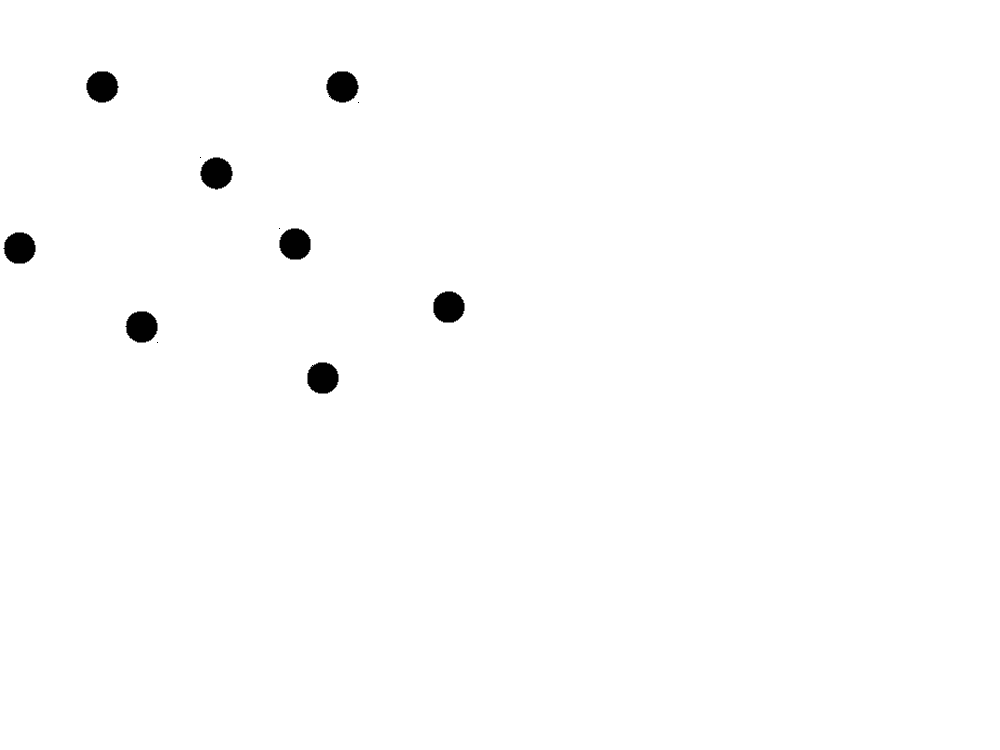
\epsfig{file = \fignet/FigSBM-Model-1.eps,
          width=.75\textwidth, clip=}    
        \onslide<3>
        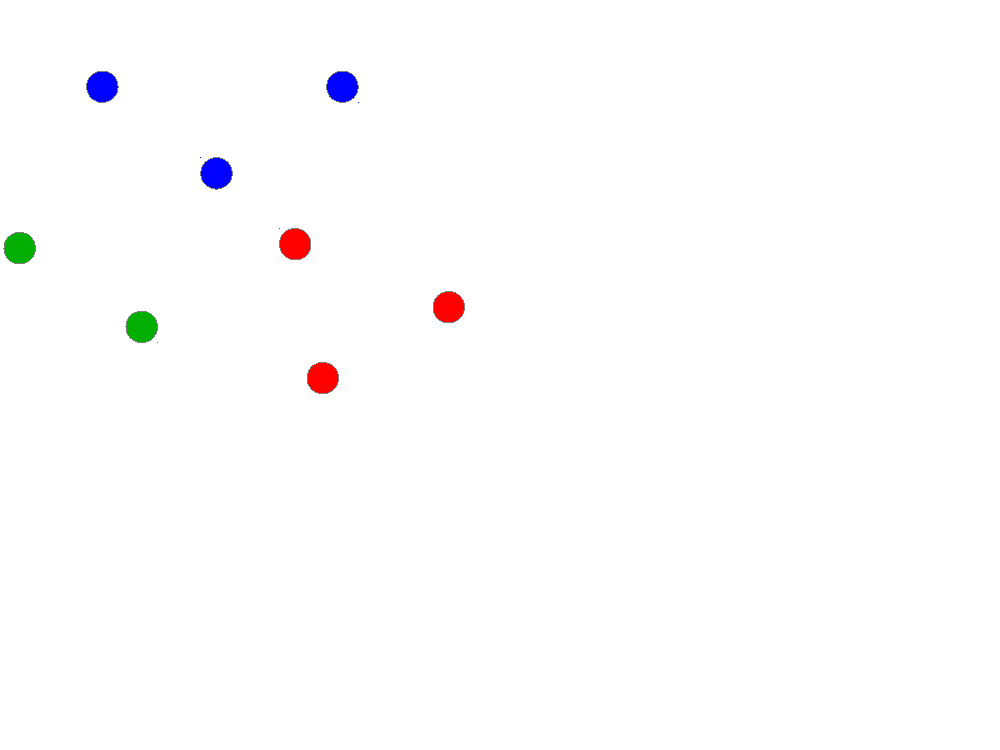
\epsfig{file = \fignet/FigSBM-Model-2.eps,
          width=.75\textwidth, clip=}    
        \onslide<4>
        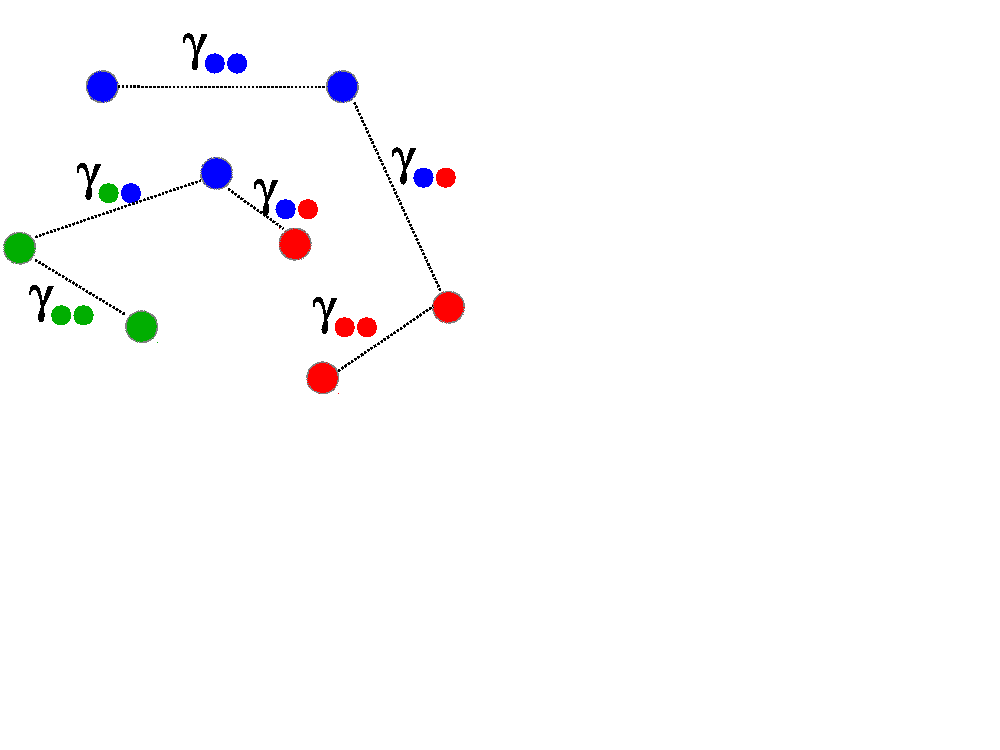
\epsfig{file = \fignet/FigSBM-Model-3.eps,
          width=.75\textwidth, clip=}    
        \onslide<5>
%        \epsfig{file = \fignet/FigSBM-Model-4.eps,
%        width=.75\textwidth, clip=}    
%        \onslide<6>
        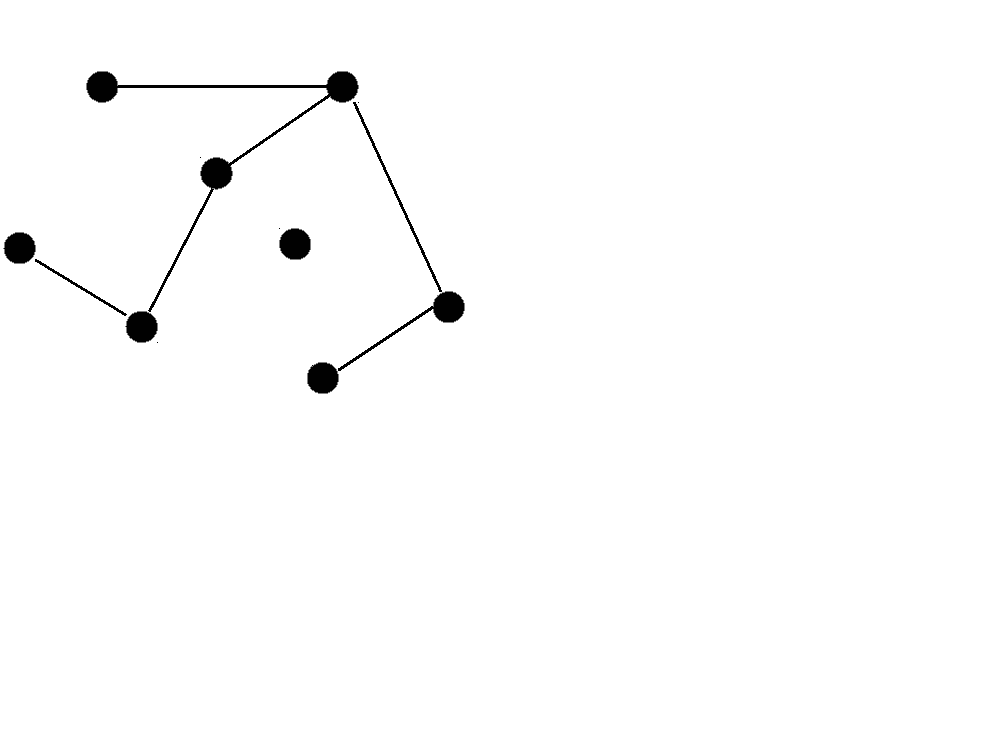
\epsfig{file = \fignet/FigSBM-Model-5.eps,
          width=.75\textwidth, clip=}    
      \end{overprint}
    \end{tabular}
  \end{tabular}
  }

%--------------------------------------------------------------------
\frame{\frametitle{Frequentist maximum likelihood inference}

  \begin{tabular}{cc}
    \hspace{-.5cm}
    \begin{tabular}{p{.5\textwidth}}
      \onslide+<1->{
        \paragraph{Maximum likelihood.} MLE of $\theta$ 
        obtained via the EM algorithm ... \\
        provided that we can calculate
        $$
        P_{\theta}(Z | X).
        $$
        ~\\~\\~\\
      }
    \end{tabular}
    & 
    \hspace{-.5cm}
    \begin{tabular}{p{.5\textwidth}}
            \begin{overprint}
        \onslide<2>
        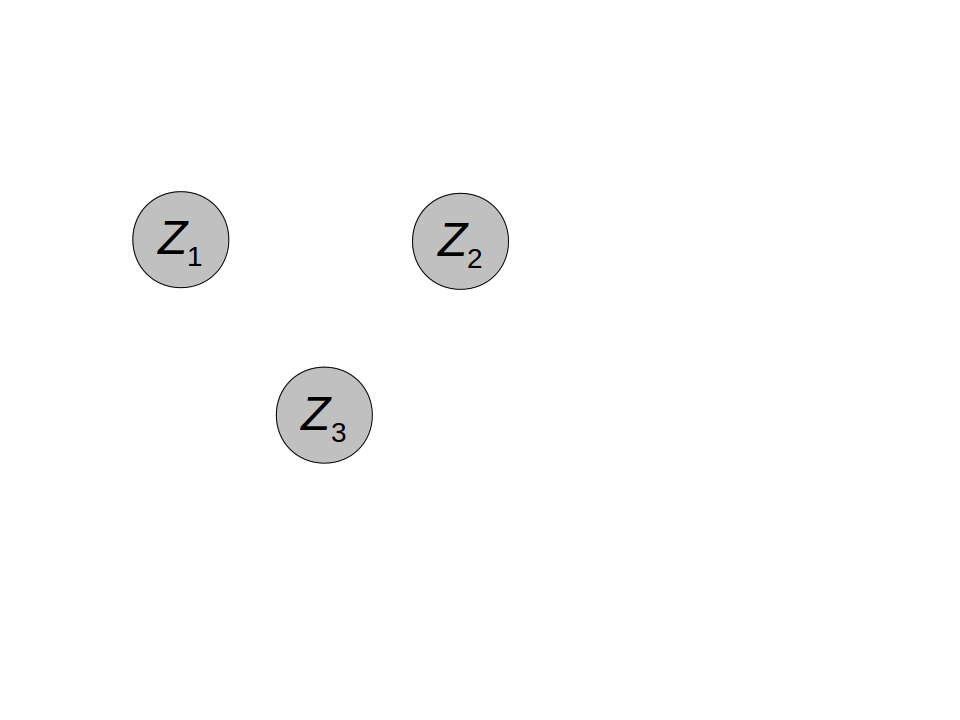
\epsfig{file=../FIGURES/FigSBM-Z.eps, clip=, width=0.6\textwidth}
        \onslide<3>
        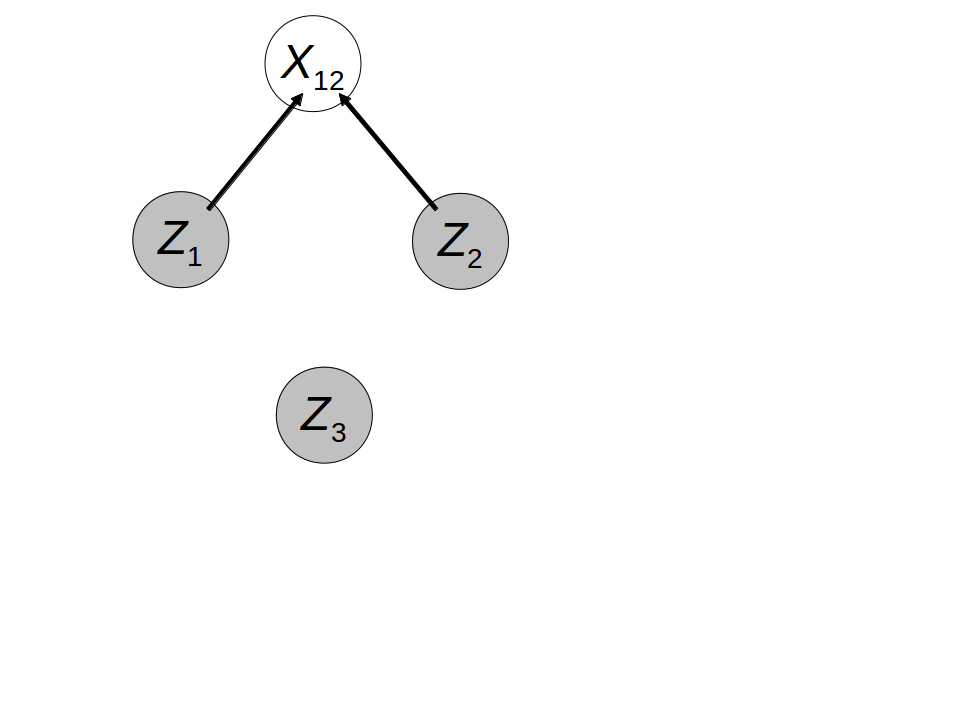
\epsfig{file=../FIGURES/FigSBM-Z-X12.eps, clip=, width=0.6\textwidth}
        \onslide<4>
        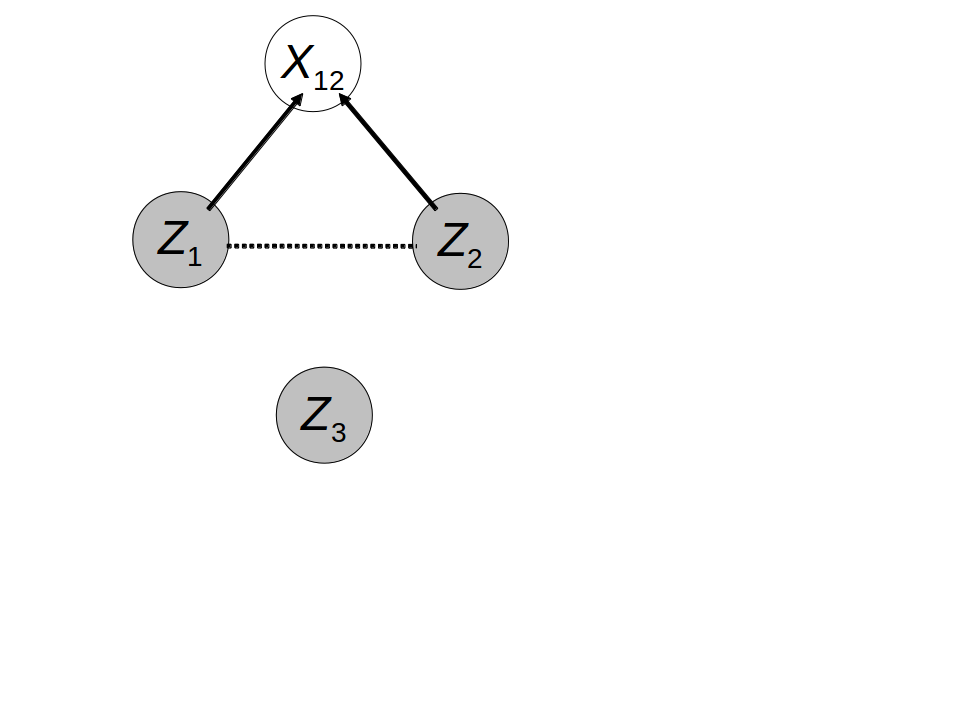
\epsfig{file=../FIGURES/FigSBM-Z-X12-Moral.eps, clip=,
          width=0.6\textwidth} 
        \onslide<5>
        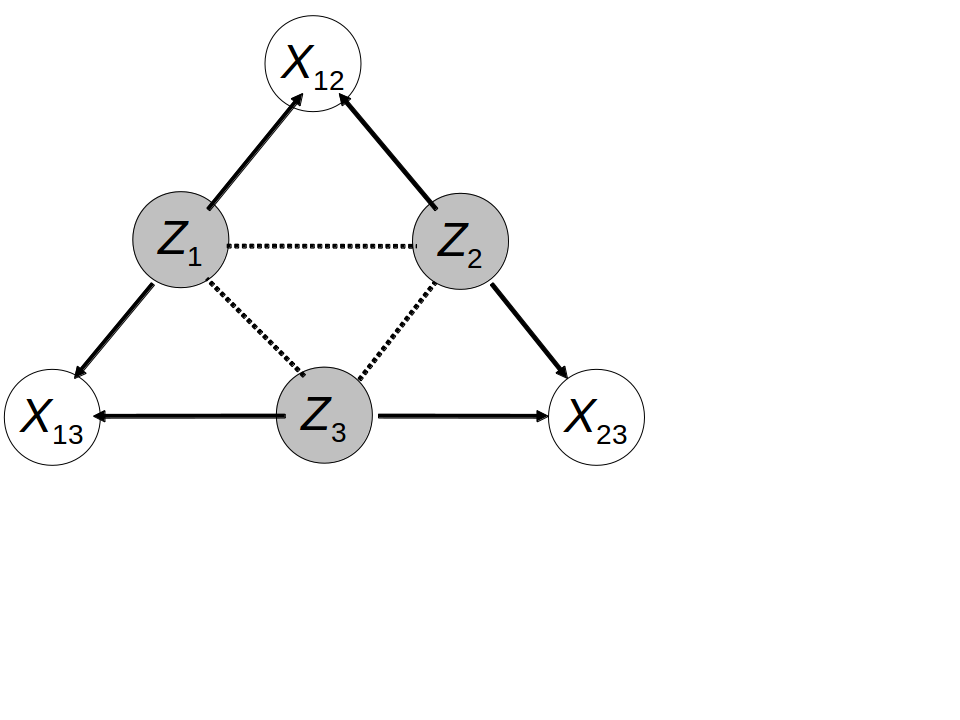
\epsfig{file=../FIGURES/FigSBM-Z-X-Moral.eps, clip=,
          width=0.6\textwidth} 
        \onslide<6->
        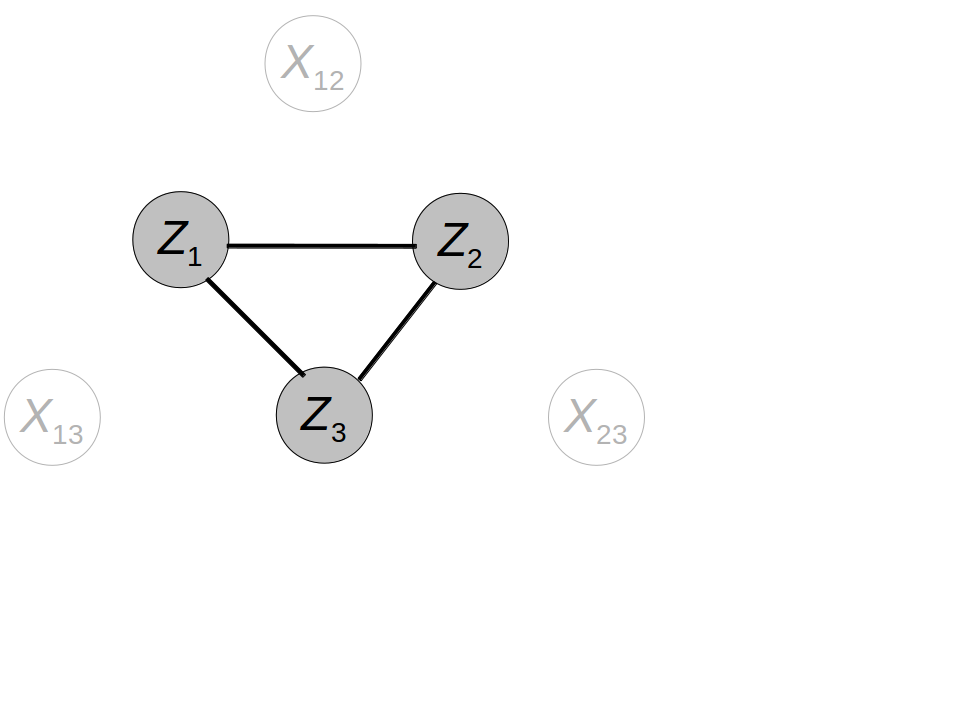
\epsfig{file=../FIGURES/FigSBM-ZcondX.eps, clip=,
          width=0.6\textwidth}
      \end{overprint}
    \end{tabular}
  \end{tabular}

  \onslide+<6->{
    \vspace{-1.5cm}
    \paragraph{Conditional distribution.} The dependency graph of
    $Z$ given $X$ is a clique. \\
    \ra No factorization can be hoped (unlike for HMM). \\
    \ra $P_{\theta}(Z | X)$ can not be computed
    (efficiently). \\
    \ra Variational techniques provide 
    $$
    Q(Z) \simeq P_{\theta}(Z | X).
    $$
  }
}

%--------------------------------------------------------------------
\frame{\frametitle{Bayesian inference}
  
  \begin{tabular}{cc}
    \hspace{-.5cm}
    \begin{tabular}{p{.5\textwidth}}
      We are now interested in 
      $$
      P(Z, \theta | X)
      $$
      \ra more intricate than $P_{\theta}(Z | X)$.
      \\~\\~\\~\\~\\
    \end{tabular}
    & 
    \hspace{-.5cm}
    \begin{tabular}{p{.5\textwidth}}
      \begin{overprint}
        \onslide<2>
        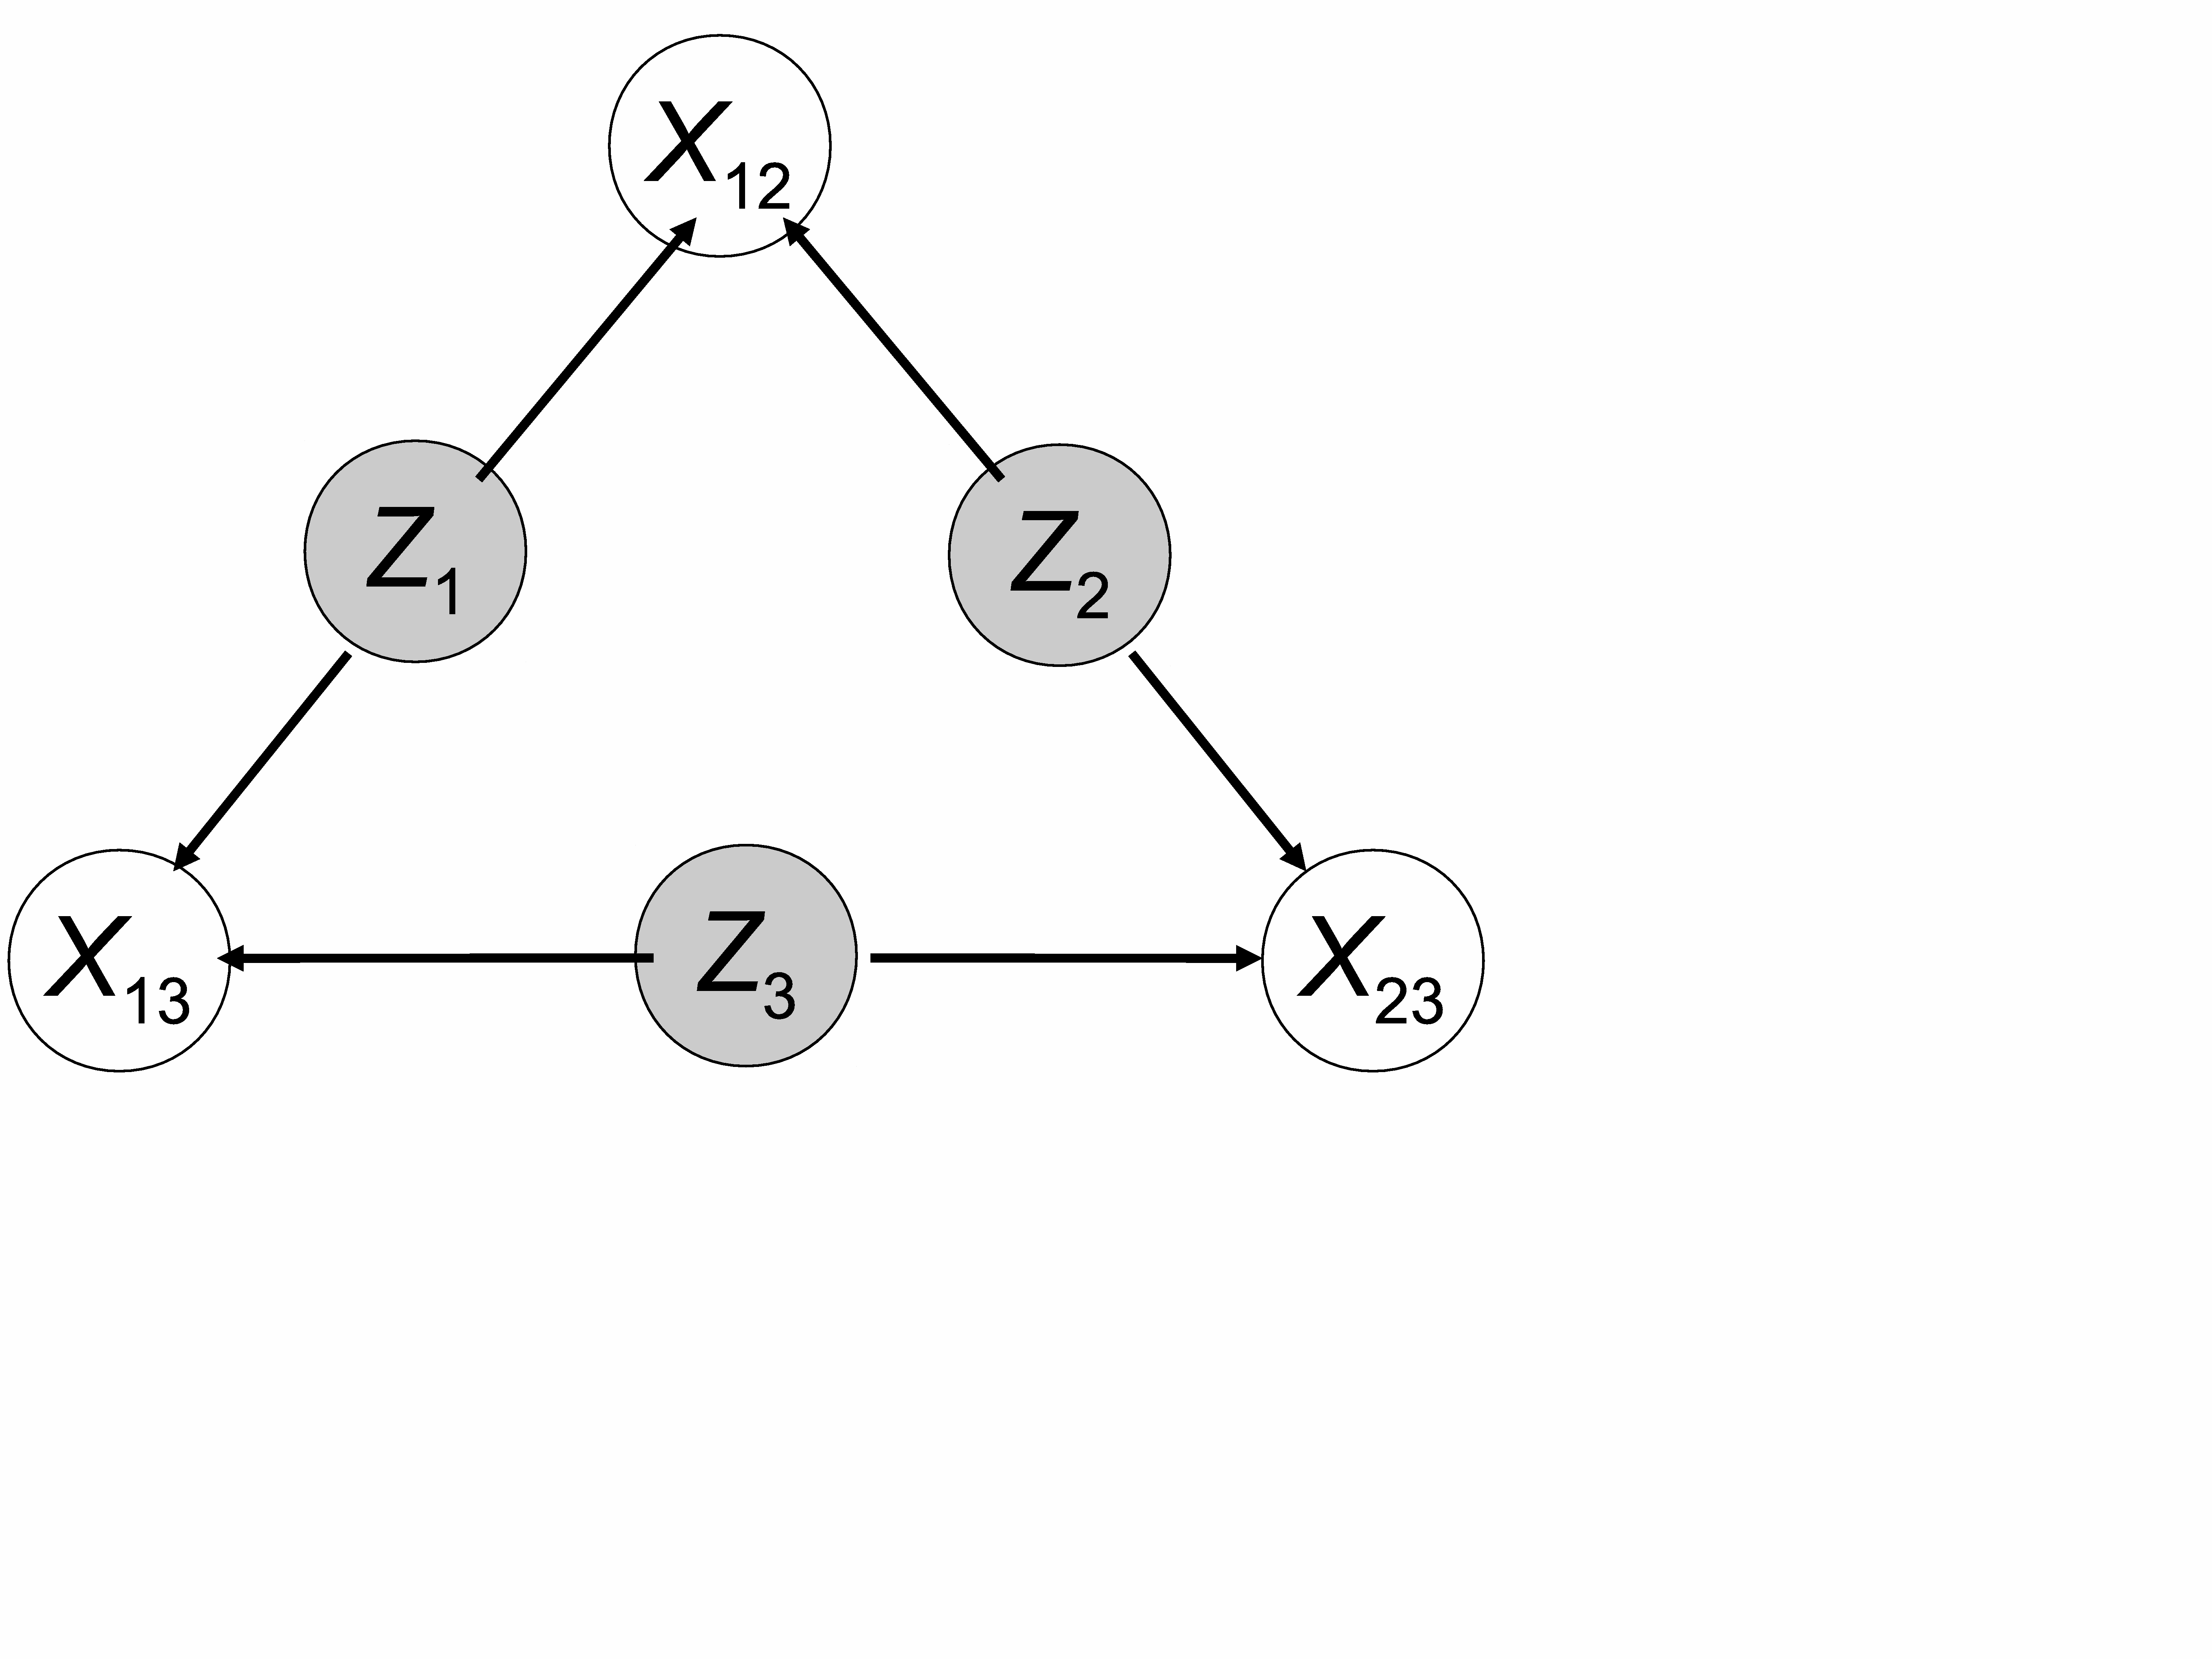
\epsfig{file = \fignet/FigSBM-Z-X.eps,
          width=.7\textwidth, clip=}   
        \onslide<3>
        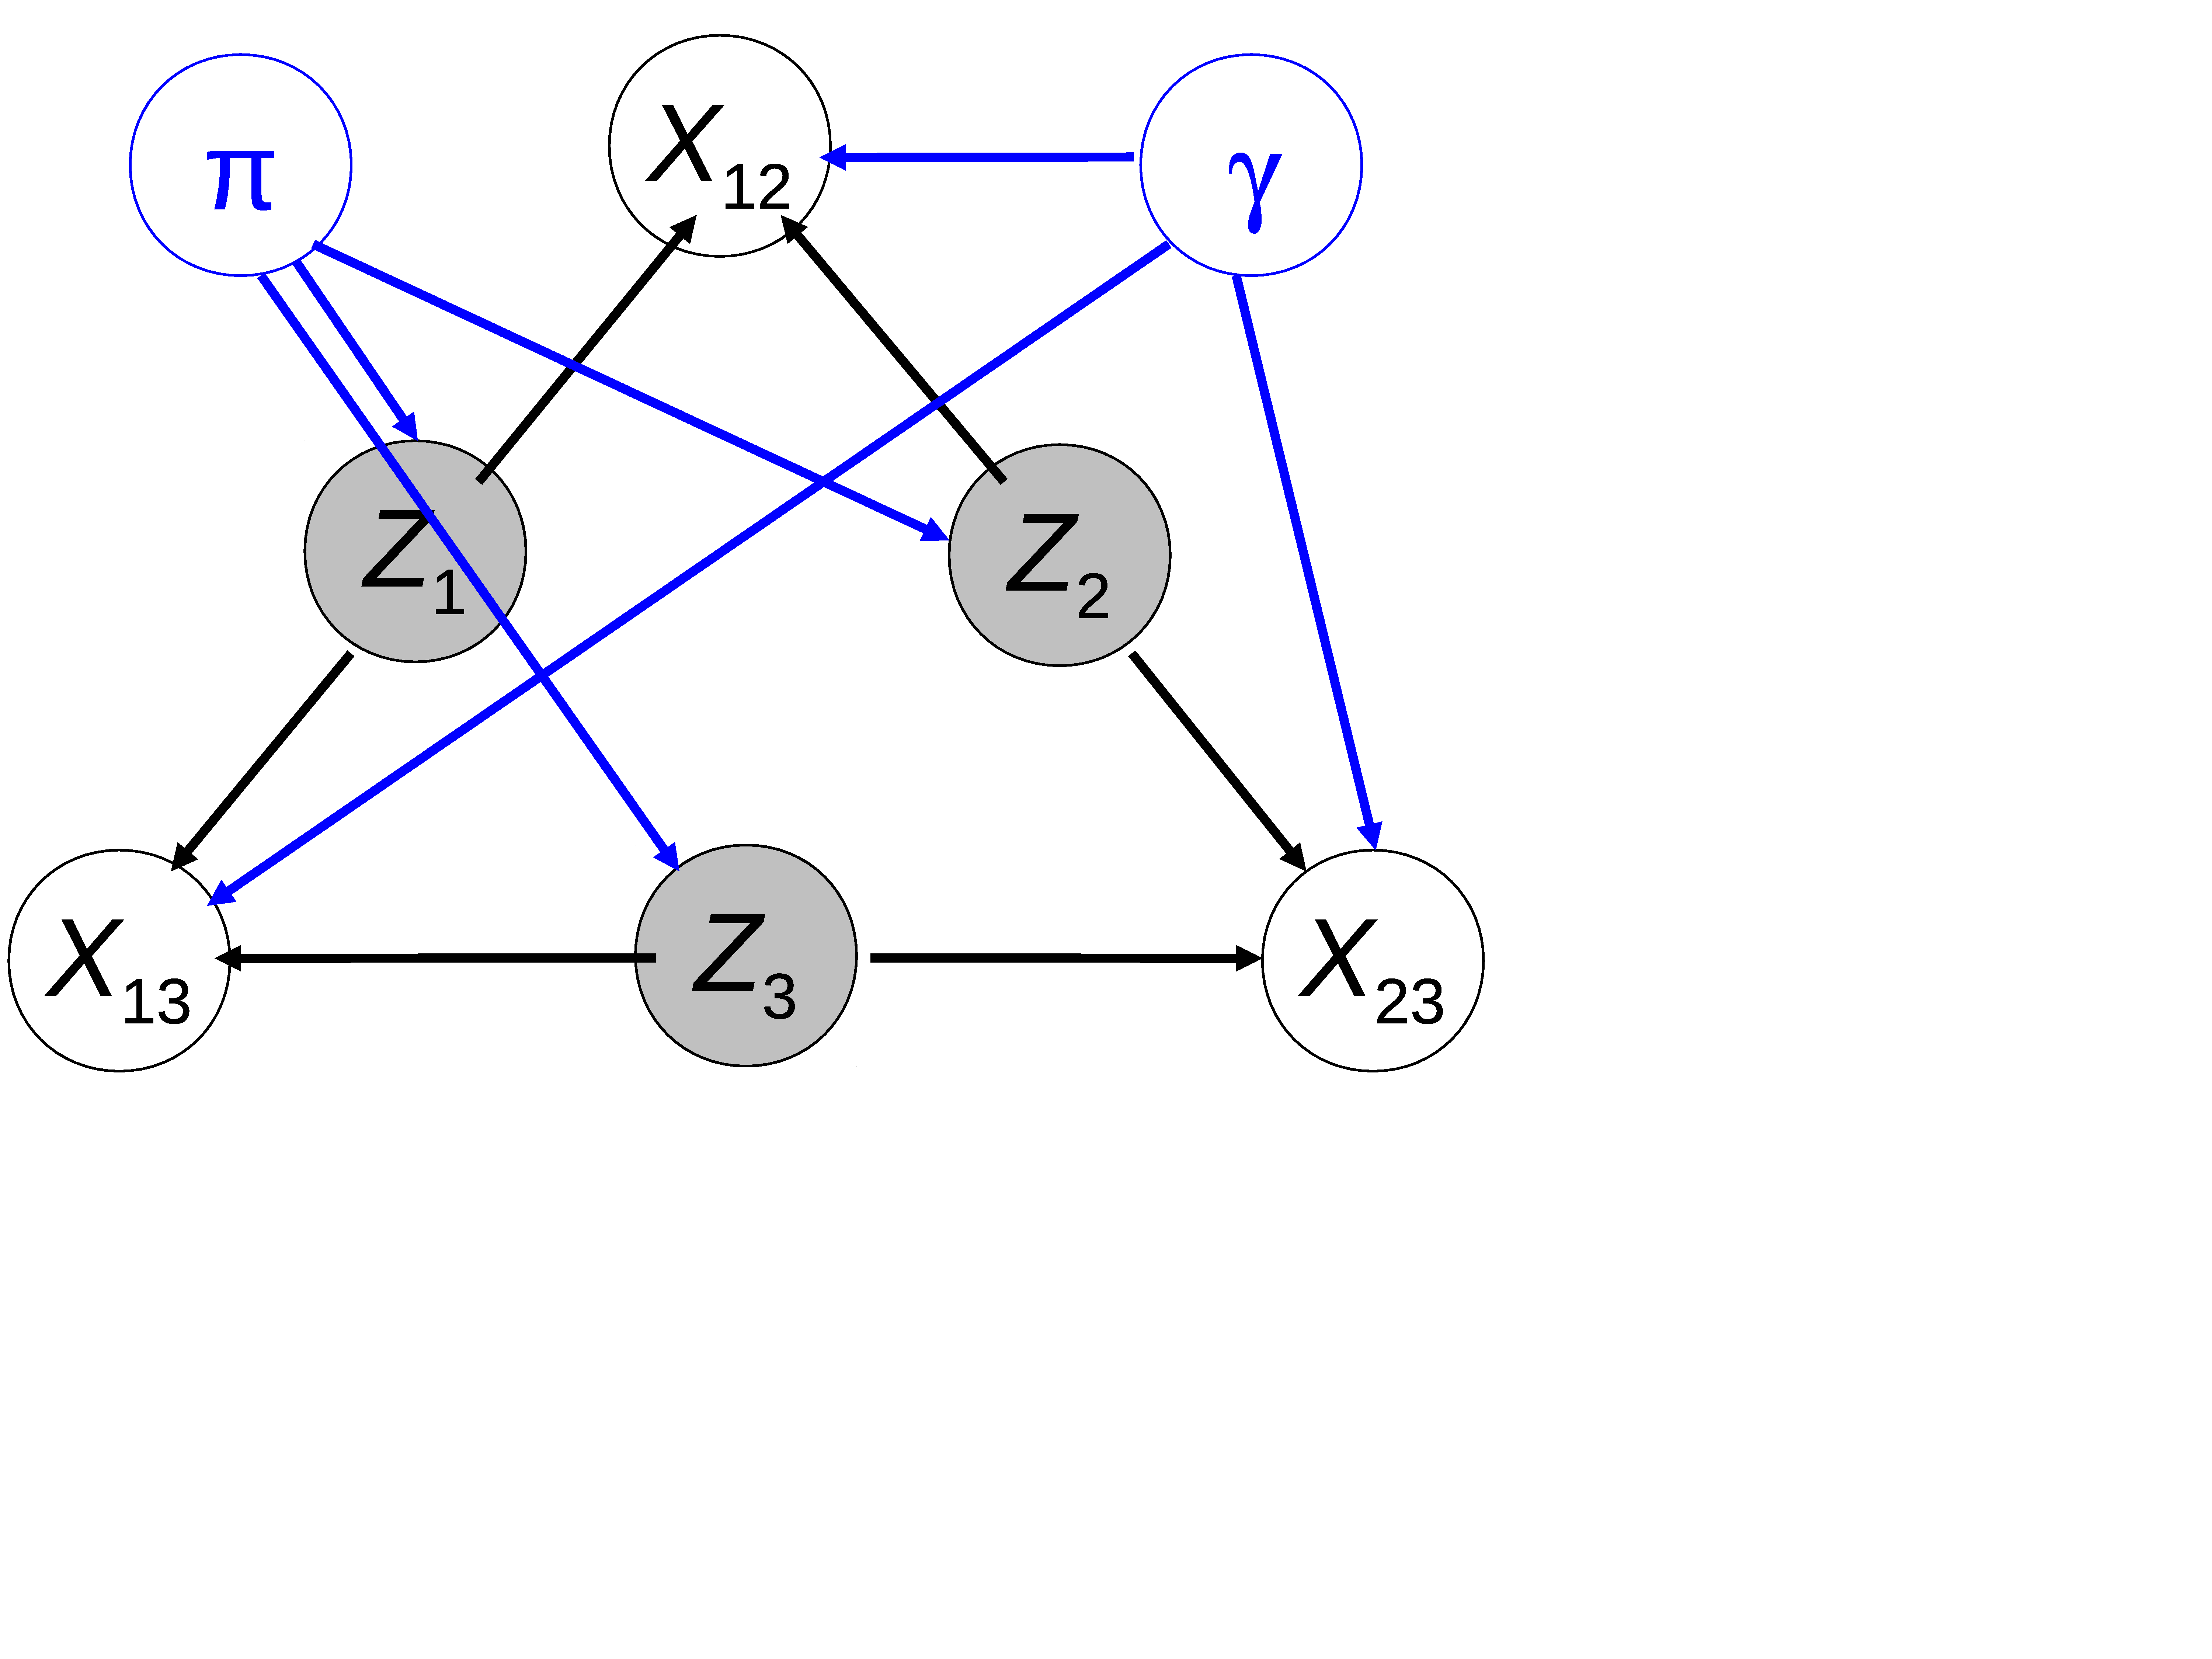
\epsfig{file = \fignet/FigSBM-Bayes-1.eps,
          width=.7\textwidth, clip=}   
        \onslide<4>
        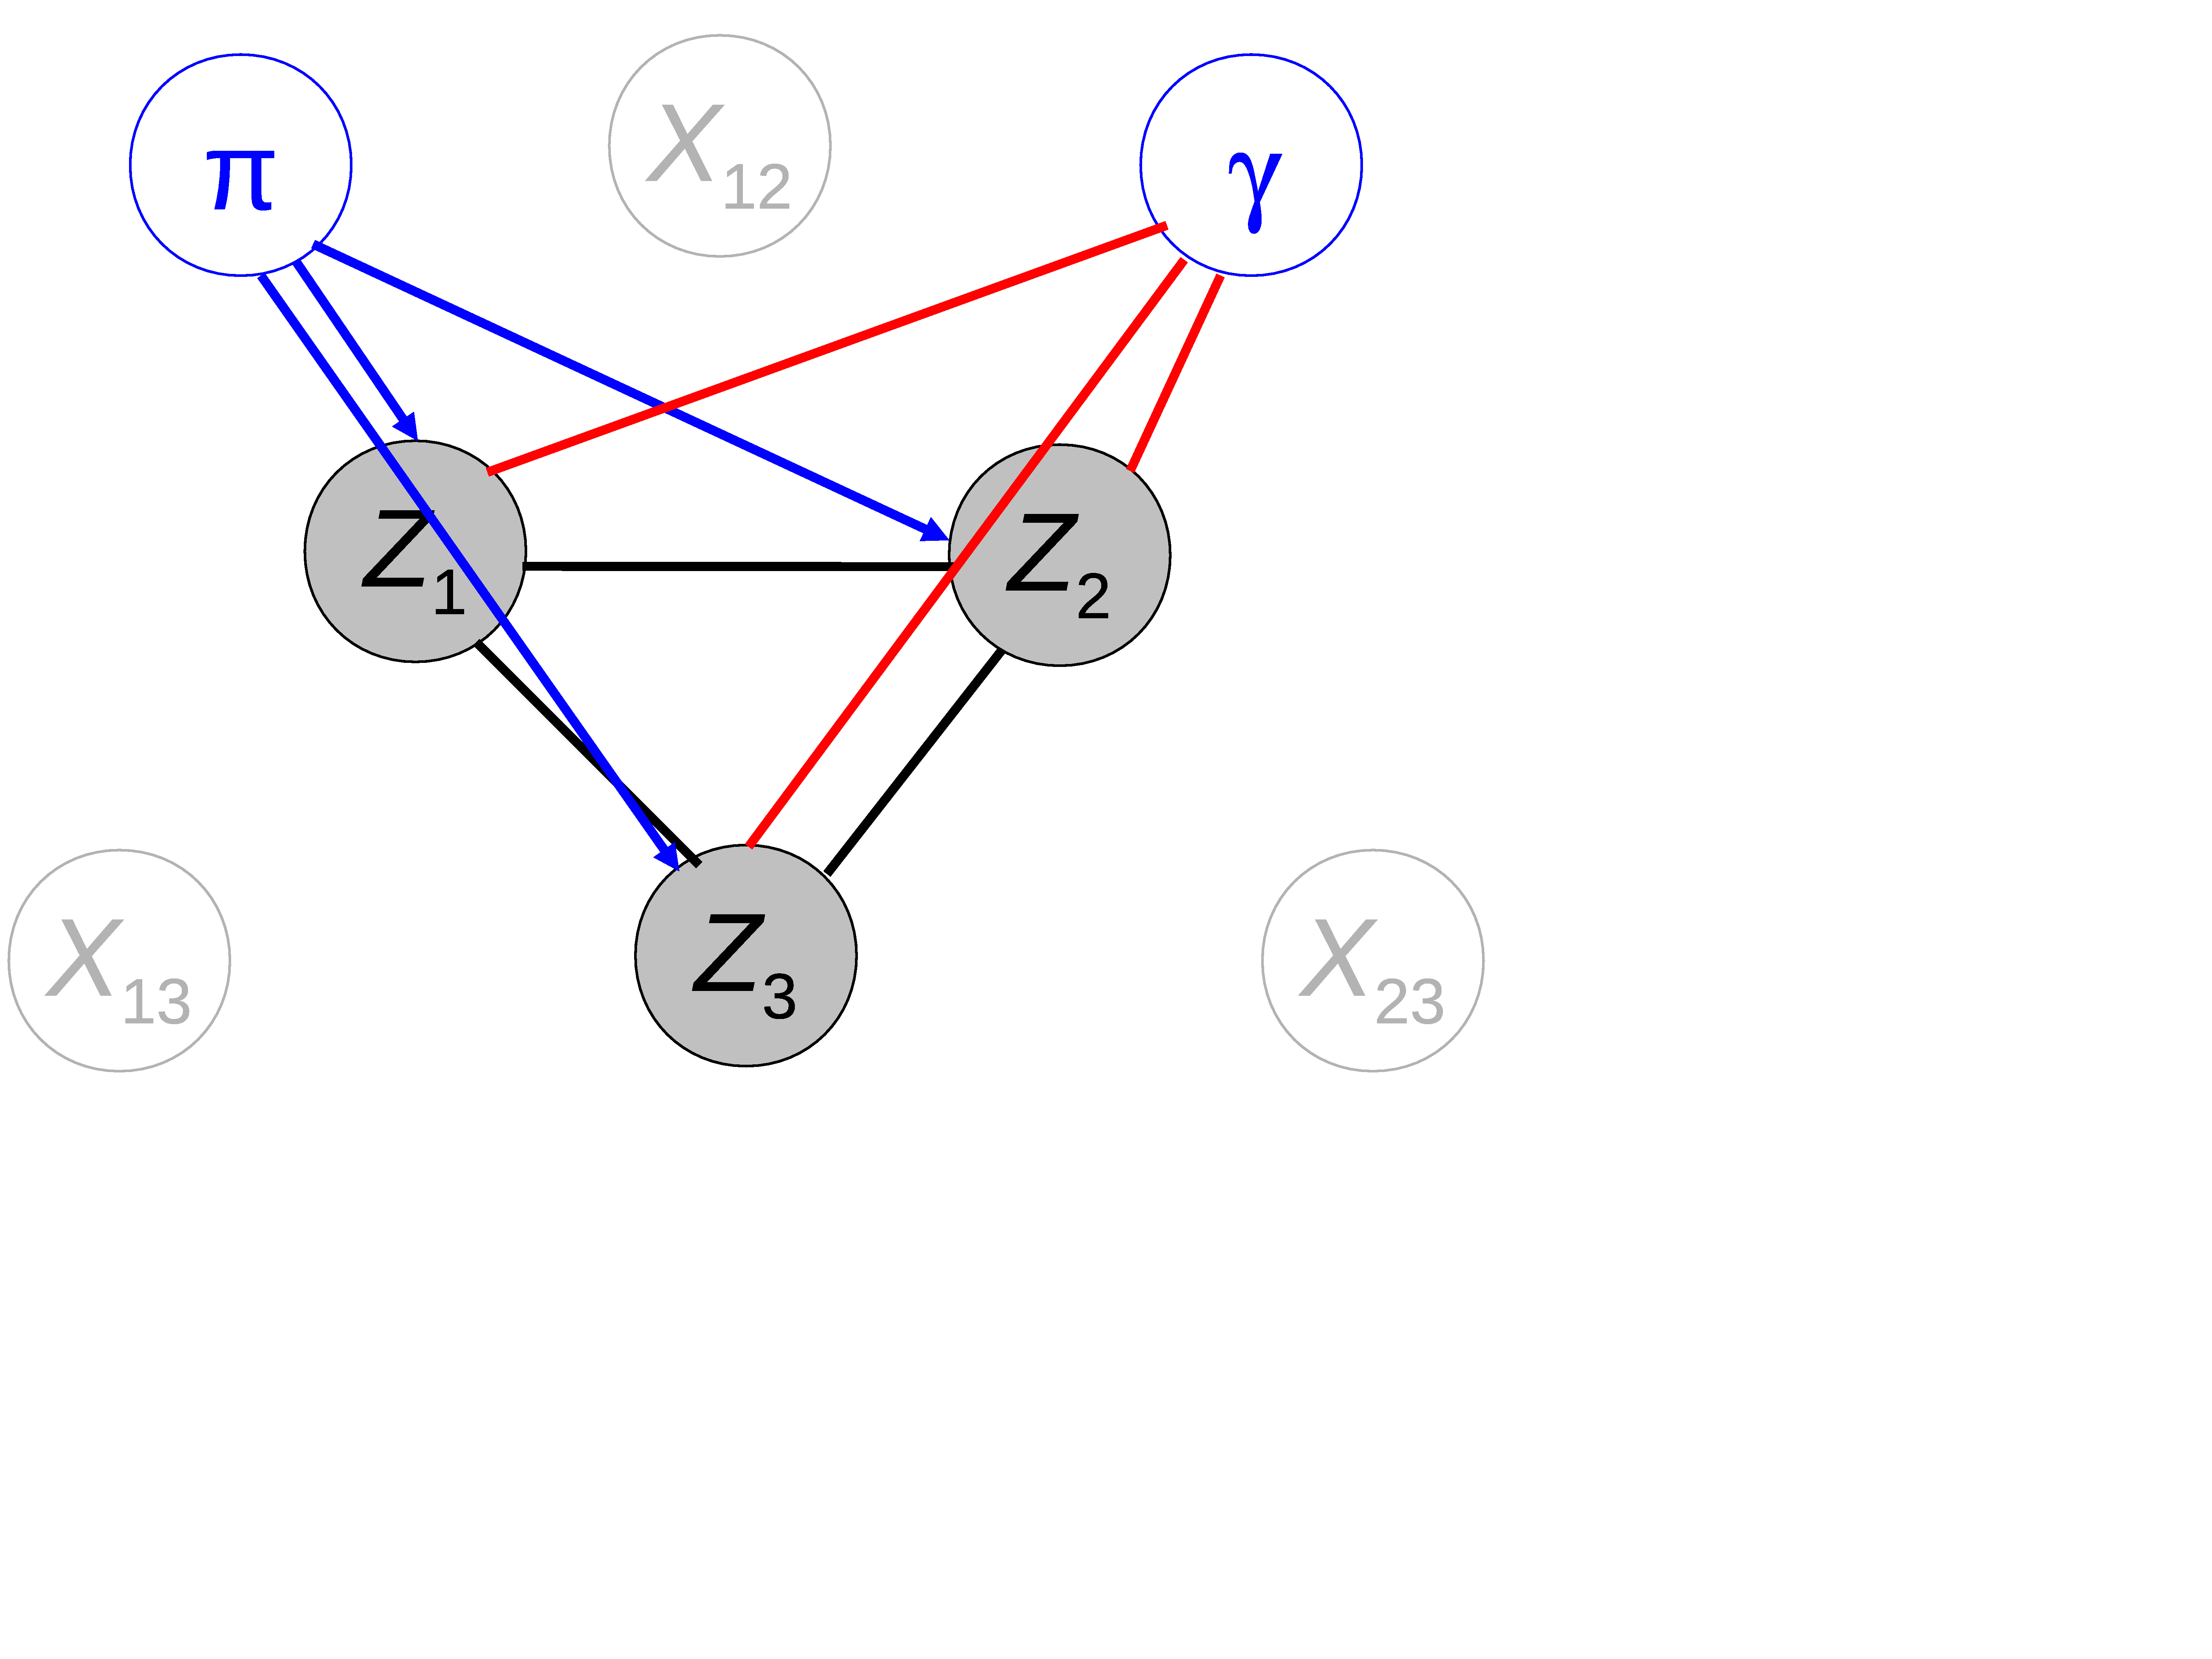
\epsfig{file = \fignet/FigSBM-Bayes-2.eps,
          width=.7\textwidth, clip=}   
      \end{overprint}
    \end{tabular}
  \end{tabular}
  
  \onslide+<4>{
    \vspace{-1cm}
    Variational techniques can provide an approximation
    $$
    Q(Z, \theta) \simeq P(Z, \theta | X).
    $$}
  }

%--------------------------------------------------------------------
%--------------------------------------------------------------------
\section[Variational approximation]{Variational approximation / Variational (Bayes) inference}
\frame{\frametitle{Variational approximation / Variational (Bayes) inference}}

%--------------------------------------------------------------------
\subsection*{Variational approximation}
%--------------------------------------------------------------------
\frame{\frametitle{K�llback-Leibler divergence}

  \paragraph{Definition.}
  $$
  KL[Q(\cdot), P(\cdot)] 
%     = \int Q \log \frac{Q}{P}  %\\
  = \Esp_Q \left( \log \frac{Q}{P} \right) %\\
  = \int Q \log Q  - \int Q \log P   
  $$

  \bigskip\bigskip\pause
  \paragraph{Some properties.}
  \begin{itemize}
  \item Not a distance, only a 'divergence'.
  \item Always positive.
  \item Null iff $P = Q$.
  \item Contrast consistent with maximum-likelihood inference.
  \end{itemize}
  }

%--------------------------------------------------------------------
\frame{\frametitle{Variational inference}

  \paragraph{Lower bound of the log-likelihood.} For any distribution
  $Q(Z)$ \refer{Jaa00,WaJ08},
  \begin{eqnarray*}
    \log P(X) & \geq & \log P(X) - KL[Q(Z),
    P(Z|X)] \\ \pause
%    & = & \log P(X; \theta) - \int Q(z) \log Q(z) \dd z
%    + \int
%    Q(z) \log P(z|X) \\
%    & = & \log P(X; \theta) - \int Q(z) \log Q(z) \dd z
%    + \int
%    Q(z) \log P(X, z) - \int Q(z) \log P(X) \dd z \\ 
    & = & \int Q(z) \log P(X, z) \dd z - \int Q(z) \log
    Q(z) \dd z \\ \pause
    & = & \Esp_Q[\log P(X, Z)] + \Hcal[Q(Z)] 
  \end{eqnarray*}
  
  \bigskip\bigskip\pause
  \paragraph{Link with EM.} This is similar to
  $$
  \log P(X) = \Esp[\log P(X, Z)|X] + \Hcal[P(Z | X)]
  $$
  replacing $P(Z|X)$ with $Q(Z)$.


  }

%--------------------------------------------------------------------
%--------------------------------------------------------------------
\subsection*{Variational inference}
%--------------------------------------------------------------------
\frame{\frametitle{Variational EM algorithm}

  \paragraph{Variational EM.} 
  \begin{itemize}
  \item M-step: compute 
    $$
    \widehat{\theta} = \arg\max_{\theta} \emphase{\Esp_{Q^*}}[\log P_{\theta}(X,
    Z)].
    $$ \\ ~\\
  \item \pause E-step: replace the calculation of $P(Z|X)$ with
    the search of
    $$
    Q^*(Z) = \emphase{\arg\min_{Q \in \Qcal} KL}[Q(Z), P(Z|X)].
    $$
    which amounts at a functional optimization problem:
    $$
    \emphase{\min_{Q \in \Qcal}} \int Q(z) \log \frac{Q(z)}{P(z|X)} \dd z.
    $$   
  \end{itemize}
  
%   \bigskip\pause
%   \paragraph{Variational Bayes EM.} Directly search for
%   $$
%   Q^*(Z, \theta) = \emphase{\arg\min_{Q \in \Qcal} KL}[Q(Z, \theta),
%   P(Z, \theta|X)].
%   $$
  }

%--------------------------------------------------------------------
\frame{\frametitle{A functional optimization problem}

  We want to minimize, \emphase{with respect to the function $Q$}, the
  functional
  $$
  \Fcal(\emphase{Q}) = \int \Lcal[\emphase{Q}(z), z] \dd z.
  $$
  
  \pause\bigskip
  \paragraph{Example.} For variational EM, take either $z =
  z$ or $z = (z, \theta)$ and set
  $$
  % \Lcal[Q(z), z] = Q(z) \log\frac{Q(z)}{P(z|X)}, 
  \Lcal[\emphase{Q}(z), z] = \emphase{Q}(z)
  \log\left[\emphase{Q}(z) / P(X, z) \right].
  $$
  
  \bigskip\pause
  \begin{theorem} \label{Thm:FuncOpt} The function 
  $$
  Q^* = \arg\min_Q \Fcal(Q)
  $$ 
  satisfies
  $$
  \forall z, \qquad \left. \frac{\partial \Lcal[Q(z),
      z]}{\partial Q(z)} \right|_{\emphase{Q^*}(z)}= 0.
  $$
  \end{theorem}

%   \paragraph{Theorem.} The function 
%   $$
%   Q^* = \arg\min_Q \Fcal(Q)
%   $$ 
%   satisfies
%   $$
%   \forall z, \qquad \left. \frac{\partial \Lcal[Q(z),
%       z]}{\partial Q(z)} \right|_{\emphase{Q^*}(z)}= 0.
%   $$

  }

%--------------------------------------------------------------------
\frame{\frametitle{Stochastic Block Model (SBM)}

  \paragraph{Likelihoods.} $Z_i =$ label, $X_{ij} = $ edge, $\theta  = (\pi, \gamma)$, $Z_{ik} = \Ibb\{i \in k\}$,
  $$
  P_{\theta}(X, Z) = 
  \prod_i \prod_k \pi_k^{\emphase{Z_{ik}}} 
  \times
  \prod_{i \neq j} \prod_{k, \ell} \underset{f_{k\ell}(X_{ij})}{\underbrace{\left[\gamma_{k\ell}^{X_{ij}} (1 - \gamma_{k\ell})^{1-X_{ij}}\right]}}^{\emphase{Z_{ik}Z_{j\ell}}}.  
  $$
%   \ra We need $P(Z_i |X)$ and $P(Z_i, Z_j|X)$.

%   \bigskip\bigskip\pause
%   \paragraph{Remark.} The conditional distribution of one label given
%   the data \emphase{+ all other labels} is
%   \begin{eqnarray*}
% %    P(Z_i | X) & \propto & \sum_{\{Z_j\}_{j \neq i}}P(Z_i,
% %    \{Z_j\}_{j \neq i}, X) \quad ... \\
%     P(Z_i = k | X, \{Z_j\}_{j \neq i}) & \propto &  \pi_k \prod_{j
%     \neq i} \prod_\ell f_{k\ell}(X_{ij})^{\emphase{Z_{j\ell}}}
%   \end{eqnarray*}
%   }

% %-------------------------------------------------------------------- 
% \frame{ \frametitle{Variational EM}

  \bigskip \pause
  \paragraph{Distribution class.} $\Qcal =$ set of \emphase{factorisable}
  distributions:
  $$
  \Qcal = \{Q: Q = \emphase{\prod_i Q_i}\}, \qquad\qquad Q_i(Z_i) = \prod_k
  \tau_{ik}^{Z_{ik}}.
  $$
  $\Rightarrow \quad Q_{ij} = Q_i Q_j$. 

  \bigskip \bigskip \pause
  Applying the theorem leads to a \emphase{fix-point} relation:
  $$
  \tau_{ik} \propto \pi_k \prod_{j \neq i} \prod_\ell
  f_{k\ell}(X_{ij})^{\emphase{\tau_{j\ell}}}
  $$
  also known as  \emphase{mean-field approximation} in physics. \refer{DPR08}
  }

%-------------------------------------------------------------------- 
\frame{ \frametitle{Application to {\sl E. coli} operon network}

%   \vspace{-0.5cm}
  \hspace{-0.5cm}
  \begin{tabular}{cc}      
    \begin{tabular}{p{0.45\textwidth}}
        \epsfig{file=\fignet/im_EcoliVEM_2.ps,
          width=.45\textwidth, clip=} 
    \end{tabular}
    &
    \hspace{-.075\textwidth}
    \begin{tabular}{p{0.45\textwidth}}
      \paragraph{Parameter estimates.} $K = 5$     \\
      \footnotesize{$\begin{array}{cccccc}
          \widehat{\gamma}_{k\ell}~(\%) & 1 & 2 & 3 & 4 & 5 \\
          \hline
          1 & . & . & . & . & . \\
          2 & 6.40 & 1.50 & 1.34 & . & . \\
          3 & 1.21 & . & . & . & . \\
          4 & . & . & . & . & . \\
          5 & 8.64 & 17.65 & . & 72.87 & 11.01 \\
          \hline
          \widehat{\pi}~(\%) & 65.49 & 5.18 & 7.92 & 21.10 & 0.30
        \end{array}$}
      \\ ~\\ 

      \onslide+<2->{
        \paragraph{Meta-graph representation.} \refer{PMD09}\\
        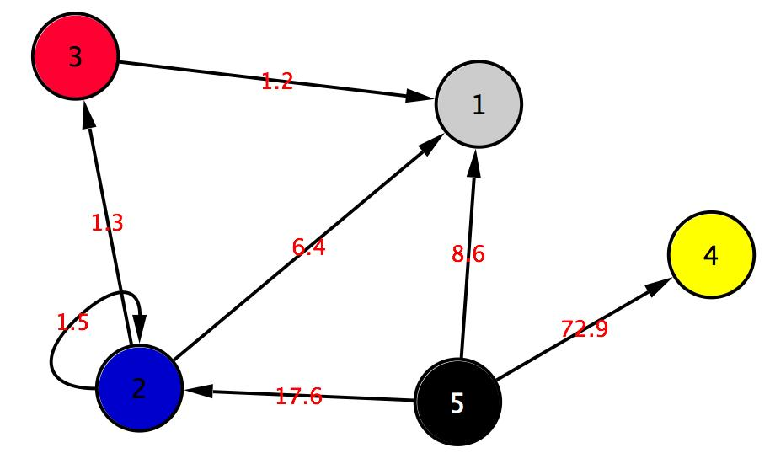
\epsfig{file=\fignet/VEMmetagraphe.ps, width=.45\textwidth, clip=}
        }
    \end{tabular}
  \end{tabular}
  }

%--------------------------------------------------------------------
\frame{\frametitle{Properties of the variational approximation}

  \emphase{Not much is known} about the quality of variational
  inference.
  \begin{itemize}
  \item VEM algorithm converges to a \emphase{different optimum than
      ML}, except for \emphase{'degenerated' models} \refer{GuB05}.
  \item Mean field approximation is asymptotically exact for models
    with infinite range dependency \refer{OpW01}.
  \end{itemize}

  \bigskip\bigskip\pause
  \paragraph{Specific case of graphs.}
  \begin{itemize}
  \item Specific asymptotic framework: \emphase{$n^2$ data, $'p' = n$
      'variables'} per individual.
  \item $P(Z|X)$ concentrates towards a Dirac mass when $n
    \rightarrow \infty$ \refer{CDP11}, \refer{MaM13}.
  \item The Dirac mass belongs to $\Qcal$...
  \end{itemize}
  }

%-------------------------------------------------------------------- 
\frame{ \frametitle{Model selection: Choice of $K$}

  \begin{itemize}
  \item Using Laplace approximation ($p = \# \text{parms}$) \refer{Sch78}:
  $$
  \BIC(K) = \log P_{\widehat{\theta}_K}(X) - \frac{p}2 \log n \approx \log P(X, K).
  $$
  \item For classification purposes (penalize for the posterior entropy: \refer{BCG00})
  $$
  \ICL(K) = \BIC(K) - \Hcal[P_{\widehat{\theta}_K}(Z|X)]
  \approx \int \Esp \left[ \log P(X, Z, \theta, K) | X\right] \dd \theta
  $$
  \end{itemize}

  \bigskip \pause
  
  \paragraph{VEM inference for SBM:}
  $$
  \widetilde{\ICL}(K) = \Esp_{Q^*} \log P_{\widehat{\theta}_K}(X, Z) - \frac{K-1}2 \log n  - \frac{K^2}2 \log n(n-1)
  $$
  $\widetilde{\BIC}(K) \simeq \widetilde{\ICL}(K)$ because $\Hcal[Q^*(Z)] \simeq 0$.

}


%--------------------------------------------------------------------
\subsection*{Variational Bayes inference}
%--------------------------------------------------------------------
\frame{\frametitle{Variational Bayes inference}

  \paragraph{Variational Bayes EM.} Directly search for
  $$
  Q^*(Z, \theta) = \emphase{\arg\min_{Q \in \Qcal} KL}[Q(Z, \theta),
  P(Z, \theta|X)].
  $$

  \bigskip \pause
  \paragraph{Exponential family / conjugate prior setting.}
  \begin{itemize}
  \item If the joint distribution $P(X, Z|\theta)$ is in the
    exponential family
    $$
    P(x, z | \theta) \propto \exp\{\emphase{\phi}(\theta)^{\transp}
    \emphase{u}(x, z)\};
    $$
  \item If the prior distribution of $\theta$ is conjugate
  \begin{eqnarray*}
    P(\theta) & \propto & \exp\{\emphase{\phi}(\theta)^{\transp} {\nu}\}
    \\    \pause 
    \Rightarrow P(x, z, \theta) & \propto &
    \exp\{\phi(\theta)^{\transp} [u(x, z) + \nu]\};
  \end{eqnarray*}
  \end{itemize}

  \bigskip\pause
  \paragraph{Class of approximate distributions.}
  \begin{itemize}
  \item If we restrict the approximate distribution $Q(Z,
    \theta)$ to
    $$
    Q \in \Qcal := \{Q: Q = \emphase{\QZ}  \emphase{\Qt}\}.
    $$
  \end{itemize}
  }

%--------------------------------------------------------------------
\frame{\frametitle{Variational Bayes EM algorithm}

  The optimal distribution $Q^*(Z, \theta) = Q^*_Z(Z) Q^*_{\theta}(\theta)$:
  $$
  Q^*(Z, \theta) = \arg\min_{Q \in \Qcal} KL(Q(Z, \theta), P(Z, \theta|X))
  $$
  satisfies the two following relations \refer{BeG03}.

  \bigskip 
  Remind that 
  $$
  \log P(X, Z, \theta) = \phi(\theta) [u(X, Z) + \nu]
  $$
  
  \bigskip 
  \paragraph{VB E-step.} 
  \begin{eqnarray*}
    \log \QZ^*(Z) %& = & \int \Qt(\theta) \log P(X, Z, \theta) \dd \theta +  \cst  \\ 
    & = & \emphase{\Esp_{Q_{\theta}}}[\log P(X, Z, \theta)] + \cst \\
    & = & \emphase{\Esp_{Q_{\theta}}}[\phi(\theta)]^\transp u(X, Z)  + \cst 
  \end{eqnarray*}
%   where $\overline{\phi} = \emphase{\Esp_{Q_{\theta}}}[\phi(\theta)]$. 

  \paragraph{VB M-step.} 
  \begin{eqnarray*}
    \log \Qt^*(\theta) & \propto & \phi(\theta)^\transp
    \left\{ \emphase{\Esp_{Q_Z}}[u(X, Z)] + \nu \right\}   + \cst 
  \end{eqnarray*}
%   where $\overline{u}(X) = \emphase{\Esp_{Q_Z}}[u(X, Z)].$
  }

%-------------------------------------------------------------------- 
\frame{ \frametitle{Application to {\sl E. coli} operon network}

  \vspace{-0.5cm}
  \hspace{-0.5cm}
  \begin{tabular}{cc}      
    \begin{tabular}{p{0.45\textwidth}}
        \epsfig{file=\fignet/im_EcoliVEM_2.ps,
          width=.45\textwidth, clip=} 
    \end{tabular}
    &
    \hspace{-0.5cm}
    \begin{tabular}{p{0.45\textwidth}}
	 \includegraphics[width=.45\textwidth]{../FIGURES/im-pi1BVEM}\\        
      \includegraphics[width=.45\textwidth]{../FIGURES/im-pi2BVEM}\\
      \includegraphics[width=.45\textwidth]{../FIGURES/im-pi3BVEM}\\
      \includegraphics[width=.45\textwidth]{../FIGURES/im-pi4BVEM}\\
      \includegraphics[width=.45\textwidth]{../FIGURES/im-pi5BVEM}\\
      \hline 
      \includegraphics[width=.45\textwidth]{../FIGURES/im-alphaBVEM}\\

    \end{tabular}
  \end{tabular}
  }

%-------------------------------------------------------------------- 
\frame{ \frametitle{Variational Bayes approximation: Simulation Study}

  Few is known about the properties of variational-Bayes inference:
  \begin{itemize}
  \item Asymptotic normality of the approximate posterior \refer{WaT04}.
  \item Consistency is proved for \emphase{some incomplete data models}
    \refer{WaT06,McT09}.
  \item In practice, VB-EM often under-estimates the posterior variances.
  \end{itemize}
  
  \bigskip\bigskip\pause
  \paragraph{Simulation design:} \refer{GDR11}
  \begin{itemize}
  \item 2-group binary SBM with parameters 
    %with 2 scenarios
    $$
    \pi=\left(\begin{array}{cc}
        0.6 & 0.4
      \end{array}\right),  
    \qquad
    \gamma=\left(\begin{array}{cc}
        0.8 & 0.2 \\
%        0.2 & \emphase{0.5/0.3}
        0.2 & 0.3
      \end{array}\right)
    $$
  % \item \pause Comparison of 4 methods: EM (when possible), {\VEM}, BP and
  %   {\VBEM}
  % \item \pause Belief Propagation (BP) algorithm: 
  %   $$
  %   \Esp_Q[\log P(X, Z)] = \sum_{i, k}
  %   \underset{\emphase{\normalsize
  %       \tau_{ik}}}{\underbrace{\Esp_Q[Z_{ik}]}} \log \pi_k + \sum_{i,
  %     j} \sum_{k, \ell} \underset{\emphase{\normalsize
  %       \Delta_{ijk\ell} \neq
  %       \tau_{ik}\tau_{j\ell}}}{\underbrace{\Esp_Q[Z_{ik} Z_{j\ell}]}}
  %   \log f(X_{ij}; \gamma_{k\ell}).
  %   $$
%  \item 500 graphs are simulated 
    for each scenario and 
    each graph size.
  \end{itemize}
  }

% %--------------------------------------------------------------------
% \frame{ \frametitle{Estimates, standard deviation and likelihood}

%   \paragraph{Comparison on small graphs ($n = 18$):}
%   {\small
%     \begin{tabular}{ccccccccc} 
%       & $\pi_1$ & $\gamma_{11}$ & $\gamma_{12}$ & $\gamma_{22}$ &
%       $\log P(X)$ \\   
%       \hline
%       \emphase{Scenario 1} & 60\% & 80\% & 20\% & 50\% & \\ 
%       \hline 
%       EM & 59.1 (13.1) & 78.5 (13.5) & 20.9 (8.4) & 50.9 (15.4) & -90.68 \\  
%       {\VEM} & 57.7 (16.6) & 78.8 (12.4) & 22.4 (10.7) & 50.3 (14.6) & -90.87\\  
%       BP & 57.9 (16.2) & 78.9 (12.3) & 22.2 (10.5) & 50.3 (14.5) & -90.85 \\  
%       {\VBEM} & 58.1 (13.3) & 78.2 (9.7) & 21.6 (7.7) & 50.8 (13.3) & -90.71 \\ 
%       \hline \\
%       \hline
%       \emphase{Scenario 2} & 60\% & 80\% & 20\% & 30\% &  \\ 
%       \hline
%       EM & 59.5 (14.1) & 78.7 (15.6) & 21.2 (8.7) & 30.3 (14.3) & -88.18 \\  
%       {\VEM} & 55.6 (19.0) & 80.1 (14.0) & 24.0 (11.8) & 30.8 (13.8) & -88.54 \\  
%       BP & 56.6 (17.8) & 80.0 (13.6) & 23.2 (11.0) & 30.8 (13.8) & -88.40 \\  
%       {\VBEM} & 58.4 (14.6) & 77.9 (12.0) & 22.3 (9.3) & 32.1 (12.3) & -88.26 \\  
%     \end{tabular} 
%     }
%   \bigskip\pause
%   \begin{itemize}
%   \item All methods provide similar results.
%   \item {\EM} achieves the best ones.
%   \item Belief propagation ({\BP}) does not significantly improve {\VEM}.
%   \end{itemize}
%   }

%--------------------------------------------------------------------
\frame{ \frametitle{{\VBEM} Credibility intervals}

  \paragraph{Actual level as a function of $n$:}   $\pi_1$: $+$,
  $\gamma_{11}$: \textcolor{red}{$\triangle$}, $\gamma_{12}$:
  \textcolor{blue}{$\circ$}, $\gamma_{22}$: \textcolor{green}{$\bullet$}
  $$
  \includegraphics[width=1\textwidth]{../FIGURES/im-ICQ2-2-new} 
  $$

  \pause \bigskip
  For all parameters, {\VBEM} posterior credibility intervals achieve the nominal level (90\%), as soon as $n \geq 30$. \\
  \ra {The {\VBEM} approximation seems to work well}.
%   \item These may be due to the concentration of $P(Z|X)$ around the
%     true value of $Z$ (work in progress).
  }

%--------------------------------------------------------------------
\frame{ \frametitle{Convergence rate of the {\VBEM} estimates}


  \paragraph{Width of the posterior credibility intervals.} \\
  \begin{tabular}{p{0.25\textwidth}p{0.25\textwidth}p{0.25\textwidth}p{0.25\textwidth}}
  \hspace{0.1\textwidth} {$\pi_1$} & 
  \hspace{0.07\textwidth}  \textcolor{red}{$\gamma_{11}$} &  
  \hspace{0.05\textwidth}  \textcolor{blue}{$\gamma_{12}$} & 
  \hspace{0.03\textwidth}  \textcolor{green}{$\gamma_{22}$} \\
  \multicolumn{4}{l}{\includegraphics[width=1\textwidth]{../FIGURES/im-ICQ2-3}}
  \end{tabular}

  \pause
  \begin{itemize}
  \item The width decreases as $1/\sqrt{n}$ for $\pi_1$.
  \item It decreases as $1/n = 1/\sqrt{n^2}$ for $\gamma_{11}$,
    $\gamma_{12}$ and $\gamma_{22}$.
  \item Consistent with the penalty of the \ICL criterion
    proposed by \refer{DPR08}.
  \end{itemize}

  \bigskip 
  Explicit inference formulas and model selection criteria for SBM: no need for Laplace approximation \refer{LBA11b} 
  }

%--------------------------------------------------------------------
%--------------------------------------------------------------------
\section{Model averaging}
\frame{\frametitle{Model averaging}}
%--------------------------------------------------------------------

%--------------------------------------------------------------------
\subsection*{Variational weights}
%--------------------------------------------------------------------
\frame{\frametitle{Bayesian model averaging}

  \paragraph{Problem.} Consider a \emphase{parameter of interest
    $\Delta$} that can be estimated with different models $\Mcal_1,
  \Mcal_2, \dots, \Mcal_K, \dots$

  \bigskip\bigskip\pause
  \paragraph{Two solutions.} 
  \begin{enumerate}
  \item Select a 'best model' $\Mcal_{\widehat{K}}$ and take
    $$
    \emphase{\widehat{\Delta}} =
    \widehat{\Delta}_{\emphase{\widehat{K}}} := \Esp(\Delta|X,
    \emphase{\widehat{K}}). 
    $$ \pause
  \item Average the estimates:
    $$
    \emphase{\widehat{\Delta}}  = \Esp(\Delta|X) = \sum_K
    P(K|X) \Esp(\Delta|X, K) =  \sum_K P(K|X)
    \emphase{\widehat{\Delta}_K}.
    $$ \pause 
    or more generally
    $$
    P(\Delta|X) = \sum_K P(K|X) P(\Delta|X, K)
    $$
  \end{enumerate}
 }

%--------------------------------------------------------------------
\frame{\frametitle{Variational weights}

  The weights $P(K|X)$ can generally not be computed
  $$
  P(K | X) = \iint P(z, \theta, K | X) \dd z \dd \theta
  $$

  \bigskip\pause 
  We can approximate the conditional $P(Z, \theta, K | X)$ with
  $$
  Q^*(Z, \theta, K) = \arg\min_{Q \in \Qcal} KL[Q(Z,
  \theta, K), P(Z, \theta, K | X)]
  $$

  \bigskip\pause
  \paragraph{Variational weights.} Taking
  $$
  \Qcal = \{Q: Q = Q_K Q_{Z|K} Q_{\theta|K}\}
  $$ \pause
  the variational approximation gives \refer{VMR12}
  \begin{eqnarray*}
    Q_K^*(K) & \propto & P(K) e^{\log P(X|K) - KL[Q^*(Z, \theta|K); P(Z,  \theta|X, K)]} \\
    & = & P(K|X) e^{-\emphase{KL[Q^*(Z, \theta|K); P(Z, \theta|X, K)]}}
  \end{eqnarray*}
  }

%--------------------------------------------------------------------
\frame{\frametitle{VBMA: the recipe}

  \paragraph{For $K = 1 \dots K_{\max}$} 
  \begin{itemize}
  \item Use regular VB-EM to compute the approximate conditional posterior 
    $$     
    Q^*_{Z, \theta|K} = Q^*_{Z|K} Q^*_{\theta|K}
    $$ 
  \item Compute the conditional lower bound of the log-likelihood
    $$     
    \log P(X|K) - KL[Q^*(Z, \theta|K); P(Z,
      \theta|X, K)] =: \log P(X|K) - KL_K.    
    $$
  \end{itemize}

  \bigskip\pause
  \paragraph{Compute the approximate posterior of model $\Mcal_K$:} 
  $$
  w_K := Q_K(K) \propto P(K | X) \exp(-KL_K).
  $$ 

  \bigskip\pause
  \paragraph{Deduce the approximate posterior of $\delta$:} 
  $$
  P(\delta | X) \approx \sum_K w_K Q^*_{\theta | K}(\delta | K)
  $$
  }

%--------------------------------------------------------------------
%--------------------------------------------------------------------
\section{From SBM to $W$-graphs}
\frame{\frametitle{From SBM to $W$-graphs}
}
%--------------------------------------------------------------------

%--------------------------------------------------------------------
\frame{\frametitle{Modeling network heterogeneity}

  \paragraph{Latent variable models} allow to capture the underlying structure of a network (e.g. SBM).

  \bigskip \bigskip \pause
  \paragraph{General setting for binary graphs.} \refer{BJR07}: %\pause
  \begin{itemize}
   \item   {A latent (unobserved) variable $Z_i$} is associated with each node:
  $$
  \{Z_i\} \text{ iid } \sim \pi 
  $$
  \item 
  Edges {$Y_{ij} = \Ibb\{i \sim j\}$ are independent conditionally} to the $Z_i$'s:
  $$
  \{Y_{ij}\} \text{ independent } | \{Z_i\}: \Pr\{Y_{ij} = 1\} = \gamma(Z_i, Z_j)
  $$
  \end{itemize}

  \bigskip 
  See \refer{MaR14} for a review.

  }


%--------------------------------------------------------------------
\frame{ \frametitle{$W$-graph model}

  \begin{tabular}{cc}
    \hspace{-.5cm}
    \begin{tabular}{p{.5\textwidth}}
	 Latent variables:
	 $$
	 (Z_i) \text{ iid } \sim \Ucal_{[0, 1]},
	 $$ ~\\
	 Graphon function $\gamma$:
	 $$
	 \gamma(z, z'): [0, 1]^2 \rightarrow [0, 1]
	 $$ ~\\    
	 Edges:
	 $$
	 \Pr\{Y_{ij} = 1\} = \gamma(Z_i, Z_j)
	 $$    
	 \end{tabular}
    & 
    \hspace{-.1\textwidth}
    \begin{tabular}{p{.5\textwidth}}
	 Graphon function $\gamma(z, z')$ \\
      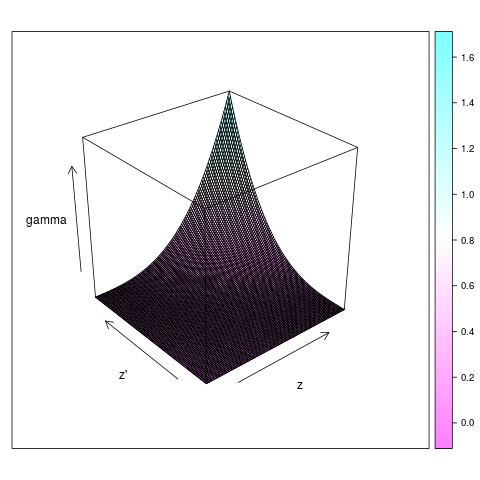
\includegraphics[width=.5\textwidth]{\fignet/FigCLADAG-W-graphon} \\
    \end{tabular}
  \end{tabular}
  
%   Intensively studied in probability theory as a limit for dense graphs \refer{LoS06}.

 }

 %--------------------------------------------------------------------
\frame{ \frametitle{Inference of the graphon function}

  \paragraph{Probabilistic point of view.}
  \begin{itemize}
   \item $W$-graph have been mostly studied in the probability literature as a limit for dense graphs: \refer{LoS06}, \refer{DiJ08}
   \item Intrinsic un-identifiability of the graphon function $\gamma$ is often overcome by imposing that $u \mapsto \int \gamma(u, v) \dd v$ is monotonous increasing.
   \item Motif (sub-graph) frequencies are invariant characteristics of a $W$-graph.
  \end{itemize}

  \bigskip \bigskip \pause
  \paragraph{Statistical point of view.}
  \begin{itemize}
   \item Not much attention has been paid to its inference until very recently: \refer{Cha12}, \refer{ACC13}, \refer{WoO13}, ...
   \item The two latter also uses SBM as a proxy for $W$-graph.
  \end{itemize}
}

%--------------------------------------------------------------------
\frame{ \frametitle{SBM as a $W$-graph model}

  \begin{tabular}{cc}
    \hspace{-.5cm}
    \begin{tabular}{p{.5\textwidth}}
	 Latent variables:
	 $$
	 (Z_i) \text{ iid } \sim \Mcal(1, \pi)
	 $$ ~\\
	 Blockwise constant graphon:
	 $$
	 \gamma(z, z') = \gamma_{k\ell}
	 $$ ~\\
	 Edges:
	 $$
	 \Pr\{Y_{ij} = 1\} = \gamma(Z_i, Z_j)
	 $$    
	 \end{tabular}
    & 
    \hspace{-.1\textwidth}
    \begin{tabular}{p{.5\textwidth}}
	 Graphon function $\gamma^{SBM}_K(z, z')$ \\
      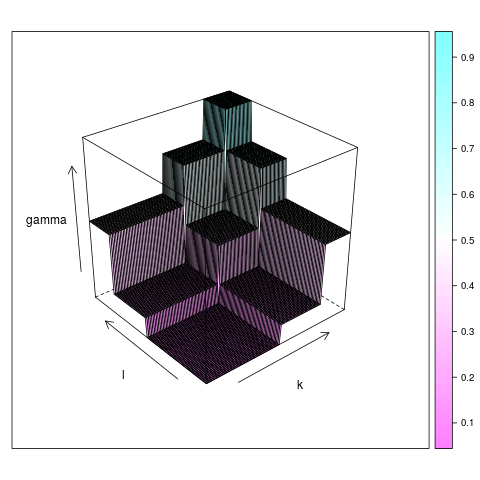
\includegraphics[width=.5\textwidth]{\fignet/FigCLADAG-SBM-graphon} \\
    \end{tabular}
  \end{tabular}

  \ra block widths $= \pi_k$, block heights $\gamma_{k\ell}$
 }

%--------------------------------------------------------------------
\subsection*{Variational Bayes inference}
%--------------------------------------------------------------------
\frame{ \frametitle{Variational Bayes estimation of $\gamma(z, z')$}

%   \paragraph{General idea.} Estimate the true $\gamma$ with a blockwise constant function $\gamma_K^{SBM}$ with $K$ classes.

  \begin{tabular}{cc}
    \hspace{-.5cm}
    \begin{tabular}{p{.5\textwidth}}
    \paragraph{VBEM inference} provides the \\approximate posteriors:
    \begin{eqnarray*}
    (\pi | X) & \approx & \text{Dir}(\pi^*) \\
    (\gamma_{k\ell} | X) & \approx & \text{Beta}(\gamma^{0*}_{k\ell}, \gamma^{1*}_{k\ell}) 
    \end{eqnarray*}
    ~
    
    \paragraph{Estimate of $\gamma(u, v)$.} 
    BEM: due \\
    to the uncertainty of the block \\
    widths, the posterior expectation \\
    of $\gamma^{SBM}_K$  is smooth
    
    \bigskip \bigskip 
    (Explicit integration using \refer{GoS10})
%     $$
%     \widehat{\gamma}_K^{SBM}(u, v) = \widetilde{\Esp}\left(\gamma_{C(u), C(v)} | Y\right)
%     $$
%     where $C(u) = 1 + \sum_k \Ibb\{\sigma_k \leq u\}$. \\ ~
%     \\
%     \refer{GoS10}
    \end{tabular}
    & 
    \hspace{-.1\textwidth}
    \begin{tabular}{p{.5\textwidth}}
	 Posterior mean ${\Esp}_{Q^*_K}(\gamma^{SBM}_K(z, z') | X)$ \\
      \includegraphics[width=.5\textwidth]{\fignet/FigGraphon-SBM-average} \\
% 	 Posterior mean of $\gamma^{SBM}_K(z, z')$ \\
%     \includegraphics[width=.6\textwidth]{../FIGURES/FigGraphon-SBM-average} \\
    \end{tabular}
  \end{tabular}
  
}

%--------------------------------------------------------------------
\frame{ \frametitle{Averaging SBMs}

  \paragraph{Model averaging:} There is no 'true $K$' in the $W$-graph model.

  \bigskip \bigskip
  \paragraph{Apply VBMA recipe.}
  For $K = 1 .. K_{\max}$, fit an SBM model via VBEM and compute
  $$
  \widehat{\gamma}_K^{SBM}(z, z') = \Esp_{Q^*_K}[\gamma_{C(z), C(z')}].
  $$
  
  \pause \bigskip \bigskip
  Perform model averaging as
  $$
  \widehat{\gamma}(z, z') = \sum_K w_K \widehat{\gamma}_K^{SBM}(z, z')
  $$
  where $w_K$ is the variational weights arising from variational Bayes inference.
%   \end{itemize}

}

%--------------------------------------------------------------------
\frame{ \frametitle{Some simulations}

  \begin{tabular}{cc}
    \hspace{-.5cm}
    \begin{tabular}{p{.5\textwidth}}
    \paragraph{Design.} Symetric graphon:
    $$
    \gamma(u, v) = \rho \lambda^2 (uv)^{\lambda-1}
    $$
    \begin{itemize}
     \item $\lambda \uparrow$: imbalanced graph 
     \item $\rho \uparrow$: dense graph
    \end{itemize}
    
    \bigskip
    \paragraph{Results.}
    \begin{itemize}
     \item More complex models as $n$ and $\lambda$ $\uparrow$
     \item Posterior fairly concentrated
    \end{itemize}

    \end{tabular}
    & 
    \hspace{-.1\textwidth}
    \begin{tabular}{p{.5\textwidth}}
    Variational posterior for $K$: $Q^*(K)$.
    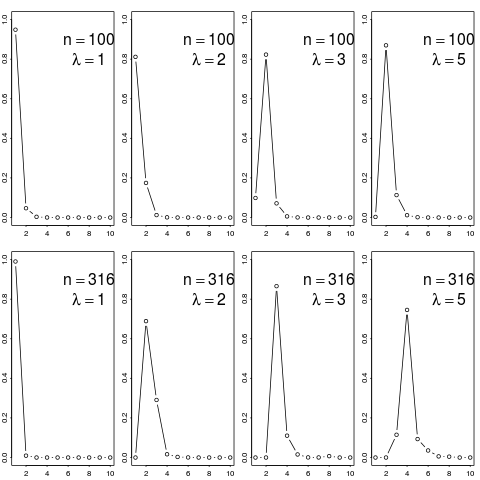
\includegraphics[width=.5\textwidth]{../FIGURES/PostDistQ-Talk-Lambda-N-rho0316227766016838}
    \end{tabular}
  \end{tabular}

}

%--------------------------------------------------------------------
\frame{ \frametitle{French political blogosphere}

  \paragraph{Website network.} French political blogs: 196 nodes, 1432 edges.
  $$
  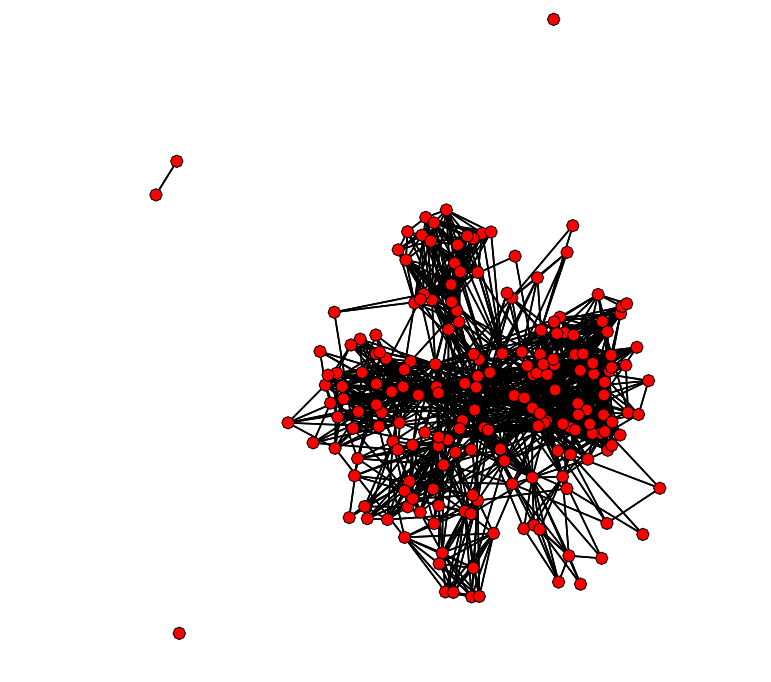
\includegraphics[width=.65\textwidth]{../FIGURES/Blogosphere-raw}
  $$
}

% %--------------------------------------------------------------------
% \frame{ \frametitle{French political blogosphere.}
% 
%   \paragraph{SBM analysis.} ~ \\
%   \vspace{-0.08\textheight}
%   \centerline{
%   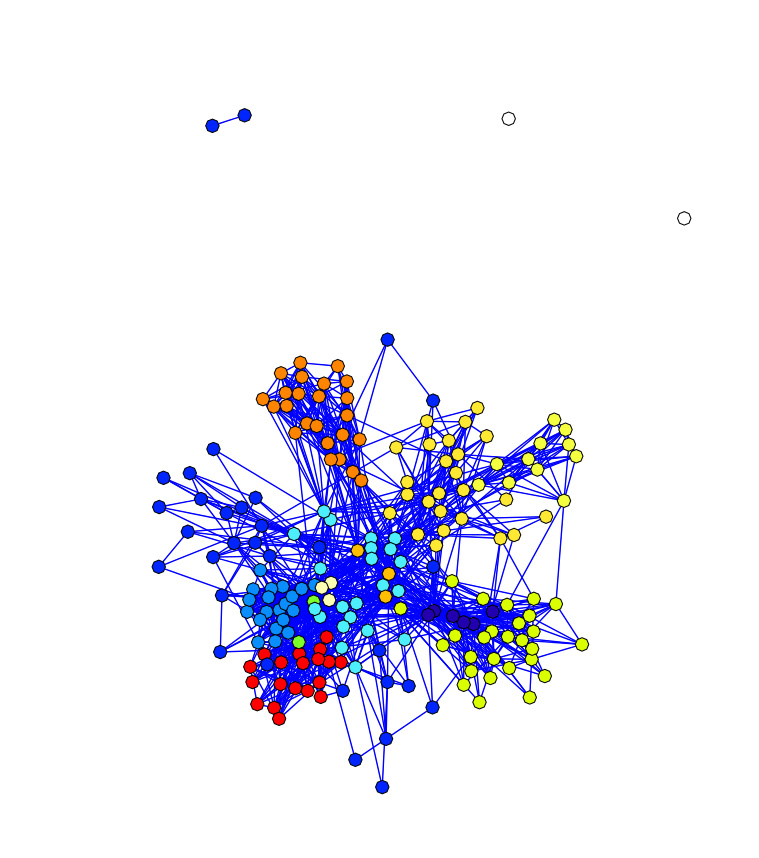
\includegraphics[width=.6\textwidth, ]{\fignet/Blogosphere-class}
%   }
% }
% 
% %--------------------------------------------------------------------
% \frame{ \frametitle{French political blogosphere}
% 
%   \paragraph{Infered graphon.} $\widehat{W}(u, v) = \Esp(\gamma(u, v) | X)$
%   \begin{overprint}
%   \onslide<1>
%   \begin{center}
%   \includegraphics[width=.5\textwidth]{../FIGURES/Blogosphere-contour}
%   \end{center}
%   \onslide<2->
%   \begin{center}
%   \includegraphics[width=.65\textwidth]{../FIGURES/Blogosphere-graphon}
%   \end{center}
%   \end{overprint}
%   Motif probability can be estimated as well as $\widehat{\mu}(m) = \Esp(\mu(m) | X)$.
% }
% 
%--------------------------------------------------------------------
\frame{ \frametitle{French political blogosphere.}

  \paragraph{Infered graphon.} $\widehat{W}(u, v) = {\Esp}_{Q^*}(\gamma(u, v))$
  \begin{center}
  %$$
  \vspace{-.1\textheight}
  \hspace{.1\textwidth}
  \includegraphics[width=.65\textwidth]{\fignet/Blogosphere-graphon}
  %$$
  \end{center}
  \pause
  \vspace{-.1\textheight}
  \paragraph{Extension to network motifs.}
  \begin{itemize}
   \item Network motifs have sociological interpretation (e.g. triangles)
   \item Motif probability can be estimated as $\widehat{\mu}(m) = {\Esp}_{Q^*}(\mu(m) | X)$ \\
   \ra Goodness of fit criterion?
  \end{itemize}
  
}


%--------------------------------------------------------------------
%--------------------------------------------------------------------
\section*{Some conclusions}
%--------------------------------------------------------------------
\frame{\frametitle{Some conclusions}

  \paragraph{Variational approximation.}
  \begin{itemize}
  \item Reasonably simple tool to get approximate conditional distributions;
  \item More scalable than standard MCMC (?);
  \item Few general theoretical guaranties;
  \item Happens to be efficient in some specific frameworks (e.g. graphs\footnote{not true for sparse graphs});
  \item Can be combined with Monte-Carlo approaches, e.g. for importance sampling \refer{LDR12}.
  \end{itemize}

  }

%--------------------------------------------------------------------
{\tiny
  \bibliography{/home/robin/Biblio/ARC,/home/robin/Biblio/AST,/home/robin/Biblio/SSB} 
  %\bibliographystyle{/home/robin/LATEX/Biblio/astats}
  \bibliographystyle{plain}
  }

%--------------------------------------------------------------------
%--------------------------------------------------------------------
\beginbackup
%-------------------------------------------------------------------- 
\section*{Appendix}

%--------------------------------------------------------------------
\frame{\frametitle{Sketch of proof}

  \begin{enumerate}
  \item \pause $Q^*$ is optimal if, \emphase{for any function $H$}
    ('perturbation', 'direction'),
    $$
    \left. \frac{\partial}{\partial t} \Fcal(Q^* +tH)\right|_{t = 0} = 0.
    $$ ~\\
  \item \pause At \emphase{$t=0$}, under regularity conditions (and
    since $(f \circ g)' = g' \times f' \circ g$)
    $$
    \frac{\partial}{\partial t} \Fcal(Q +tH) 
    = \int \frac{\partial}{\partial t} \Lcal[Q(z)+tH(z), z]
    \dd z 
    = \int H(z) \frac{\partial \Lcal[Q(z), z]}{\partial
      Q(z)} \dd z.
    $$ ~\\
  \item \pause The '\emphase{fundamental lemma} of variation calculus'
    says that
    $$
    \forall h, \; \int f(z) h(z) \dd z = 0  \qquad
    \Rightarrow \qquad \forall z, \; f(z) = 0.
    $$
  \end{enumerate}
  }

%--------------------------------------------------------------------
\frame{\frametitle{Variational optimization}

  We want to minimize $KL[Q(Z, \theta), P(Z, \theta |
  X)]$ \emphase{within $\Qcal$}, that is
  $$
  \Fcal(\QZ, \Qt) = \int \int \QZ(z) \Qt(\theta) \log
  \frac{\QZ(z) \Qt(\theta)}{P(X, z, \theta)} \dd z \dd
  \theta.
  $$

  \bigskip\pause
  To get the optimal $\QZ^*$, we set
  $$
  \Lcal_Z[\emphase{\QZ}(z), z] = \emphase{\QZ}(z) \int
  \Qt(\theta) \log \frac{\emphase{\QZ}(z) \Qt(\theta)}{P(X, z,
    \theta)} \dd \theta.
  $$

  \bigskip\pause 
  According to Theorem \ref{Thm:FuncOpt}, $\QZ^*$ satisfies
  $$
  \frac{\partial \Lcal_Z[\emphase{\QZ}(z), z]}{\partial
    \emphase{\QZ}(z)} = \int \Qt(\theta) \log
      \frac{\Qt(\theta)}{P(X, z, \theta)} \dd \theta +
      \log \emphase{\QZ}(z) - 1 = 0
  $$
  }

%--------------------------------------------------------------------
\frame{ \frametitle{Influence of the graph size}
  Comparison of \textcolor{red}{{\VEM}: $\bullet$} and
  \textcolor{blue}{{\VBEM}: $+$} \\
  %in scenario 2 (most difficult). \\
  Left to right: $\pi_1$, $\gamma_{11}$, $\gamma_{12}$, $\gamma_{22}$.

  \bigskip
  \emphase{Means.} \\
  \includegraphics[width=1\textwidth]{../FIGURES/im-etudnVB1} \\
  
  \pause
  \emphase{Standard deviations.} \\
  \includegraphics[width=1\textwidth]{../FIGURES/im-etudnVB2}
  
  \begin{itemize}
  \item {\VBEM} estimates converge more rapidly than {\VEM} estimates.
  \item Their precision is also better.
  \end{itemize}
  }

%--------------------------------------------------------------------
\subsection*{Classification}
%--------------------------------------------------------------------
\frame{\frametitle{Classification with HMM}

  \begin{tabular}{cc}
    \hspace{-.5cm}
    \begin{tabular}{p{.45\textwidth}}
      \onslide+<1->{
        \paragraph{Context.} A 2-state (normal/alert) HMM where the
        'normal' distribution if known.
      }
      
      \onslide+<2->{
        \bigskip
        \paragraph{Model.}
        \begin{itemize}
        \item $X_t|Z_t=0 \sim \phi$
        \item $X_t|Z_t=1 \sim g = \sum_k \pi_k f_k$
        \end{itemize}
      }
      
      \onslide+<3->{
        \bigskip
        \paragraph{Classification}
        $$
        \tau_t = \Pr\{Z_t = 1 | X\}
        $$
        $\widehat{\tau}_K$ for a $K$-component mixture.
      }
    \end{tabular}
    & 
    \hspace{-.5cm}
    \begin{tabular}{p{.5\textwidth}}
      \onslide+<1->{
        \paragraph{Influenza incidence rate:} Weekly data. \\
        \epsfig{file = \figbma/Grippe-Norm.eps, 
          height=.5\textwidth, width=0.5\textheight,  clip=,
          angle=270} \\
        \\
         (R\'eseau sentinelle).
        }
    \end{tabular}
  \end{tabular}
}

%--------------------------------------------------------------------
\frame{\frametitle{Classification with HMM}

  \begin{tabular}{cc}
    \hspace{-.5cm}
    \begin{tabular}{p{.45\textwidth}}
      \onslide+<1->{
        \paragraph{Mixture emission.} For each $K$, estimates of
        \textcolor{blue}{$g$} and \textcolor{green}{$\tau$} are obtained.
      }

      \onslide+<9->{
        \bigskip
        \paragraph{Model averaging.}
        $$
        \widehat{\tau} = \sum_K w_K \widehat{\tau}_K
        $$
        }
    \end{tabular}
    & 
    \hspace{-.5cm}
    \begin{tabular}{p{.5\textwidth}}
      \begin{overprint}
        \onslide<2>
        \epsfig{file = \figbma/Grippe-NormHist.eps, 
          height=.5\textwidth, width=0.5\textheight,  clip=, angle=270} \\
        \onslide<3>
        \epsfig{file = \figbma/Grippe-Mixt-K1.eps,
          height=.5\textwidth, width=0.5\textheight, clip=, angle=270} \\   
        \onslide<4>
        \epsfig{file = \figbma/Grippe-Mixt-K2.eps,
          height=.5\textwidth, width=0.5\textheight, clip=, angle=270} \\   
        \onslide<5>
        \epsfig{file = \figbma/Grippe-Mixt-K3.eps, 
          height=.5\textwidth, width=0.5\textheight, clip=, angle=270} \\  
        \onslide<6>
        \epsfig{file = \figbma/Grippe-Mixt-K4.eps, 
          height=.5\textwidth, width=0.5\textheight, clip=, angle=270} \\  
        \onslide<7>
        \epsfig{file = \figbma/Grippe-Mixt-K5.eps, 
          height=.5\textwidth, width=0.5\textheight, clip=, angle=270} \\  
        \onslide<8>
        \epsfig{file = \figbma/Grippe-Mixt-K6.eps, 
          height=.5\textwidth, width=0.5\textheight, clip=, angle=270} \\  
        \onslide<9->
        \epsfig{file = \figbma/Grippe-Mixt-BMA.eps, 
          height=.5\textwidth, width=0.5\textheight,  clip=, angle=270} 
      \end{overprint}
    \end{tabular}
  \end{tabular}
  
  \onslide+<10->{
    \bigskip
    The estimation of $\tau_t$ provides a control of the FDR under
    dependency \refer{SuC09}:
    $$
    \widehat{FDR}(s) = \frac{\sum_{t: \widehat{\tau}_t \leq s}
      \widehat{\tau}_t}{\# \{t: \widehat{\tau}_t \leq s\}}.
    $$
  }
}

%--------------------------------------------------------------------
%--------------------------------------------------------------------
\backupend
%--------------------------------------------------------------------

%--------------------------------------------------------------------
%--------------------------------------------------------------------
\end{document}
%--------------------------------------------------------------------
%--------------------------------------------------------------------

  \begin{tabular}{cc}
    \hspace{-.5cm}
    \begin{tabular}{p{.5\textwidth}}
    \end{tabular}
    & 
    \hspace{-.5cm}
    \begin{tabular}{p{.5\textwidth}}
    \end{tabular}
  \end{tabular}
